\documentclass[letterpaper,12pt]{book}
\usepackage[spanish]{babel}
\decimalpoint 
\usepackage[utf8]{inputenc}
%\usepackage{ifpdf}            %provee un switcheado facil para pdf o dvi
%\usepackage[numbers]{natbib}  %para la bibliografia
\usepackage{cite}
%\usepackage{gnuplottex} %por si se quisiera usar gnuplot directamente



\usepackage{lscape} 
\usepackage{epsfig}
\usepackage{graphics}
\usepackage{graphicx}
\usepackage{amsfonts}  
\usepackage{multicol}
\usepackage{wrapfig}   
%\usepackage[lofdepth,lotdepth]{subfig}%subs clasificados en lof y lot
%\usepackage{subfig}%subs clasificados en lof y lot
\usepackage{textcomp} 
\usepackage{subfloat} 
\usepackage{float}
%\usepackage{placeins}% provides \FloatBarrier, it prevents floats from being moved over it. 
\usepackage{multirow}
\usepackage{amsmath}
\usepackage{amssymb} 
\usepackage{bm}
\usepackage{color} %Para poner letras con color
\usepackage{soul} %Subrayar.
\usepackage[normalem]{ulem}
\usepackage[usenames,dvipsnames]{xcolor} %Definir nombres de colores
\usepackage{url} %Para escribir urls
\usepackage{listings} %Para transcribir código
\usepackage{footnote} %Para poner footnotes en floats
\usepackage{array}
\usepackage{mathrsfs} %Font cursivo
\usepackage{enumerate}
\usepackage[T1]{fontenc}

%\usepackage{tocloft}

\usepackage[lined,boxed,commentsnumbered, algochapter]{algorithm2e}
%\usepackage{setspace}%Reducir el espacio en la biblio
%\renewcommand{\bibfont}{\small}%Letra pequeña en la biblio


%\usepackage{enumitem}%reducir espacio de items
%\setlist[1]{itemsep=-3pt}
 
% \usepackage{cleveref}
% %\crefname{section}{§}{§§}
% \crefname{section}{§}{§§}
% \Crefname{section}{§}{§§} 

%\usepackage{framed} %%%Not using it.    

%\usepackage{cite} %%%Not working

\usepackage{titlesec}         %para titulos fancy de capitulos
\usepackage{caption}  
\captionsetup[figure]{margin=0.5cm,font=small,labelfont=bf}
\captionsetup[table]{margin=0.5cm,font=footnotesize,labelfont=bf}
\captionsetup[lstlistlisting]{margin=0.5cm,font=footnotesize,labelfont=bf}
\captionsetup[algorithmcf]{margin=0.5cm,font=footnotesize,labelfont=bf}


\usepackage[list=true]{subcaption}
\captionsetup[subfigure]{margin=0.5cm,font=footnotesize,labelfont=bf}
\captionsetup[subtable]{margin=0.5cm,font=footnotesize,labelfont=bf}


%\usepackage{psfrag}             %para que texto en la figura sea remplazado
                                %incluso formulas
\usepackage[inner=3.2cm,outer=2.5cm, top=4.5cm, bottom=2.0cm]{geometry}
\usepackage[final]{pdfpages}    %para que meta facilmente paginas de pdf's

\usepackage{booktabs} %Fancy toprule, midrule, bottomrule
\usepackage{tabularx}           %tablas con anchos establecidos
\usepackage{makeidx}    %para que haga un indice de palabras. Notar:

%\usepackage{nextpage}\pagestyle{headings}
\usepackage{fancyhdr}           %para las lineas de los headers
\pagestyle{fancy}               %idem
\setlength\voffset{-0.7in}
\fancyheadoffset[LE,RO]{15pt}
%\setlength\headsep{25pt}


% Dutch style of paragraph formatting, i.e. no indents. 
\setlength{\parskip}{1.3ex plus 0.2ex minus 0.2ex}
\setlength{\parindent}{0pt}

% %******************************************************
%Mis librerías Blas

%theorem & proof packages
\newtheorem{theorem}{Theorem}[section]
\newtheorem{proposicion}[theorem]{Proposición}
\newtheorem{corolario}[theorem]{Corolario} 
\newenvironment{proof}[1][Dem]{\begin{trivlist} %proof
\item[\hskip \labelsep {\bfseries #1}]}{\end{trivlist}}
\newcommand{\qed}{\nobreak \ifvmode \relax \else %qed
      \ifdim\lastskip<1.5em \hskip-\lastskip
      \hskip1.5em plus0em minus0.5em \fi \nobreak
      \vrule height0.75em width0.5em depth0.25em\fi}

% %******************************************************

% %* Número de cuenta
% \newcommand{\alumnocta}[1]{\def\elalumnocta{#1}}
% %* Jefe(a) de la División de Estudios Profesionales
% \newcommand{\jefeDEP}[1]{\def\eljefeDEP{#1}} 
% %* Nombre de la carrera               
% \newcommand{\nomcarrera}[1]{\def\elnomcarrera{#1}}
% %* Sinodal propietario A
% \newcommand{\sinoda}[1]{\def\elsinoda{#1}}
% %* Sinodal suplente A
% \newcommand{\suplea}[1]{\def\elsuplea{#1}}
% %* Sinodal propietario B
% \newcommand{\sinodb}[1]{\def\elsinodb{#1}}
% %* Sinodal suplente B  
% \newcommand{\supleb}[1]{\def\elsupleb{#1}}
% %* Jefe(a) del Consejo Departamental de la carrera
% \newcommand{\jefeCD}[1]{\def\eljefeCD{#1}}


% \alumnocta{40802391-7***}
% \jefeDEP{El Jefe(a) de la División de Estudios Profesionales}  %--'
% \nomcarrera{Física}
% \sinoda{El Sinodal A}
% \suplea{El Suplente A}
% \sinodb{El Sinodal B}
% \supleb{El Suplente B}
% \jefeCD{El Jefe(a) del Consejo Departamental de \elnomcarrera}

\newcommand{\titulo}{Working title on portada}
\newcommand{\titulito}{Working title on headers}
\newcommand{\nombre}{{\Large \textbf{\textsc{Blas Kolic}}}}
\newcommand{\carrera}{{\large \textsc{Físico}}}
\newcommand{\director}{{\large\textsc{Dr. Fancy Pants}}}
\newcommand{\fecha}{2017} 

%%%%%%%%%%%%%%%%%%%%%%%%%%%%%%%%%%%%%%%%%%%%%%%%%%%%%%%
%% Para asegurar que no ponga encabezados en las páginas blancas al
%% final de los capítulos que terminan en página impar.

\makeatletter
\def\cleardoublepage{\clearpage
\if@twoside
  \ifodd\c@page\else
    \hbox{}
    \thispagestyle{plain} %cambiar a empty para que no ponga el numero de pag.
    \newpage
    \if@twocolumn\hbox{}\newpage\fi
  \fi
\fi}
\makeatletter

%%%%%%%%%%%%%%%%%%%%%%%%%%%%%%%%%%%%%%%%%%%%%%%%%%%%%%%%%
%%Algunos otros detalles de fancyheaders, como pie de pagina en el exterior,
%%y que en paginas impares el titulo del capitulo se muestre a la derecha
%%y en italicas (Definicion del estilo de pagina)
\pagestyle{fancy}
\fancyhf{}
\renewcommand{\chaptermark}[1]{\markboth{ \emph{#1}}{}}
\fancyhead[LO]{}
\fancyhead[RE]{\leftmark}
\fancyfoot[LE,RO]{\thepage}


%%%%%%para activar, poner despues de \begin(document)%%%%%%%%%%%%%

%%%%%%%%%%%%%%%%%%%%%%%%%%%%%%%%%%%%%%%%%%%%%%%%%%%%%%%%%%%%%%%%

\makeindex              %hay que correr makeindex archivo.idx y luego compilar

\setlength{\headheight}{16pt} %para que no se queje por fancyheaders
\setlength{\marginparwidth}{1.5cm} %para que todonotes sea util en este caso
\definecolor{dark-red}{rgb}{0.4,0.15,0.15}
\definecolor{dark-blue}{rgb}{0.15,0.15,0.4}
\definecolor{medium-blue}{rgb}{0,0,0.5}
\definecolor{dark-green}{RGB}{50,71,13}

\ifpdf
\usepackage[pdfauthor={Kolic Blas},%
pdftitle={\titulito},%
pdftex]{hyperref} %este TIENE que ser el ultimo comando aqui
\hypersetup{   %para que aparezcan o no los cuadros de los links
  linktocpage,%make page number, not text, be link 
  colorlinks,%
  citecolor=dark-blue,%
  filecolor=black,%
  linkcolor=dark-green,%
  urlcolor=NavyBlue
  % menucolor
  % runcolor
  % anchorcolor
}
\else
  \usepackage[dvipdfm]{hyperref}
  \hypersetup{   %para que aparezcan o no los cuadros de los links
    colorlinks,%
    citecolor=dark-blue,%
  %    citecolor=black,%
    filecolor=black,%
    linkcolor=dark-red,%
  %    linkcolor=black,%
    urlcolor=black
  }
\fi

%\renewcommand{\sectionautorefname}{\S}
\def\sectionautorefname{\S$\!$}
\def\subsectionautorefname{\S$\!$}
\def\subsubsectionautorefname{\S$\!$}


\begin{document}

%%%%%%%%%%%%%%%%% DEFINICION DE COMANDOS %%%%%%%%%%%%%%%%%

\newcommand{\polk}[1]{\sum_{k=0}^n #1 x^k}
\newcommand{\polj}[1]{(\sum_{j=0}^k #1 )}
\newcommand{\pk}{{^{n}P_{\mathbb{K}}}}
\newcommand{\pkn}[1]{{^{n}P_{\mathbb{C}}^ #1 }}
\newcommand{\algpol}{\mathcal{A}(^{n}P_{\mathbb{K}},+,\cdot)}
\newcommand{\ball}[1]{B_{#1,\bm{x}_0}(\bm{\mu})}
\newcommand{\norm}[1]{\left\lVert#1\right\rVert}
\newcommand{\afc}[1]{\hat{\Psi}^{\dagger}_#1}
\newcommand{\afa}[1]{\hat{\Psi}_{#1}}
\newcommand{\anni}[1]{\hat{a}_{#1}}
\newcommand{\crea}[1]{\hat{a}_{#1}^{\dagger}}
\newcommand{\interact}[4]{\afc{#1}\afc{#2}\afa{#3}\afa{#4}}
\newcommand{\bra}[1]{\left\langle #1\right|}
\newcommand{\ket}[1]{\left|#1\right\rangle}
\newcommand{\tens}{\mathbin{\mathop{\otimes}}}

\newcommand{\ketB}[1]{\big|#1\big\rangle}
\newcommand{\braket}[2]{\left\langle #1\middle|#2\right\rangle} 
\newcommand{\braketB}[2]{\big\langle #1 \big|#2\big\rangle} 
\newcommand{\nubar}{\bar{\nu}}
\newcommand{\nutau}{\nu_{\tau}}
\newcommand{\numu}{\nu_{\mu}}
\newcommand{\nue}{\nu_e}
\newcommand{\numubar}{\bar{\nu}_{\mu}}
\newcommand{\nuebar}{\bar{\nu}_e}
\newcommand{\dmtwo}{\Delta m^2}
\newcommand{\stt}{\sin^2{ 2 \theta}}
\newcommand{\numunue}{\numu \rightarrow \nue}
\newcommand{\numunuebar}{\numubar \rightarrow \nuebar}
\newcommand{\pspace}{\left(\sin^2{ 2 \theta}, \Delta m^2\right)}
\newcommand{\pplane}{\sin^2{ 2 \theta}\mbox{--}\Delta m^2}
\newcommand{\bs}[1]{\boldsymbol{#1}}
\newcommand{\data}{\boldsymbol{D}}
\newcommand{\bgr}{\boldsymbol{B}}
\newcommand{\signal}{\boldsymbol{S}}
\newcommand{\pred}{\boldsymbol{Q}}
\newcommand{\enuqe}{E_{\nu}^{QE}}
\newcommand{\like}{\mathscr{L}}
%\newcommand{\true}{\Delta \mathscr{L_{\mathbf{V}}}}
\newcommand{\true}{\Delta \mathscr{L}}
\newcommand{\fake}{\Delta \like_{\mathbf{f}\ i}^{\{\bs{p}_0\}}}
\newcommand{\eff}{\chi^2_{\mathbf{Ef}}}%no me gusta esta notacion!!!!
\newcommand{\NF}{n_{\mathbf{f}}}
\newcommand{\critic}{\Delta\like^{\{\bs{p}_0\}}_c}


\newcommand\scalemath[2]{\scalebox{#1}{\mbox{\ensuremath{\displaystyle #2}}}}





%%%float parameters
\renewcommand{\topfraction}{0.85}
\renewcommand{\textfraction}{0.1}
\renewcommand{\floatpagefraction}{0.75}
% %%%Puse esto para los float se queden hasta arriba cuando les toca


% \makeatletter
% \setlength{\@fptop}{0pt}
% \makeatother


%\renewcommand{\contentsname}{Contenido}
\renewcommand{\bibname}{Bibliografía}
\renewcommand{\indexname}{Índice}
\renewcommand{\figurename}{Figura}
\renewcommand{\tablename}{Tabla}
\renewcommand{\listtablename}{Índice de tablas}
\renewcommand{\chaptername}{Capítulo}
\renewcommand{\appendixname}{Apéndice}
\renewcommand\lstlistingname{Código}
\renewcommand\lstlistlistingname{Código}
\renewcommand{\algorithmcfname}{Algoritmo}
\renewcommand{\listalgorithmcfname}{Índice de algoritmos y código}
%\renewcommand{\algorithmautorefname}{algoritmo}

\setcounter{tocdepth}{2}%Para que salga hasta 3=subsubsection,
                        %4=paragraph, en el índice general. 

\makeatletter
\providecommand\phantomsection{}% for hyperref

\newcommand\listofillustrations{%
    \chapter*{Índices de figuras, tablas, algoritmos y código}%
    \phantomsection
    \addcontentsline{toc}{chapter}{Índices de figuras, tablas,
      algoritmos y código}%
    \section*{Figuras}%
    \phantomsection
    \addcontentsline{toc}{section}{\protect\numberline{}Figuras}%
    \@starttoc{lof}%
    \bigskip
    \section*{Tablas}%
    \phantomsection
    \addcontentsline{toc}{section}{\protect\numberline{}Tablas}%
    \@starttoc{lot}
    \section*{Algoritmos y código}%
    \phantomsection
    \addcontentsline{toc}{section}{\protect\numberline{}Algoritmos y código}%
    \@starttoc{loa}%
    \bigskip
}
\makeatother

%\hyphenation{pa-la-bra}         %para que separe correctamente palabra
% usar \- entre silabas y en el mismo texto para evitar probs. con acentos

%%%Comandos para cambiar los identificadores en itemize
%\renewcommand{\labelitemi}{$\bullet$}
%\renewcommand{\labelitemii}{$\cdot$}
%\renewcommand{\labelitemiii}{$\diamond$}
%\renewcommand{\labelitemiv}{$\ast$}
%%%

%%% Posiblemente util para hacer una especie de itemize
%\begin{description}
%\item[Biology] Study of life.
%\item[Physics] Science of matter and its motion.
%\item[Psychology] Scientific study of mental processes and behaviour.
%\end{description}
%%%

% \tiny
% \scriptsize
% \footnotesize
% \small 	
% \normalsize
% \large 	
% \Large 	
% \LARGE 	
% \huge 	
% \Huge



%%%%%%%% Modifica formato de los titulos de los capitulos %%%%%%%

\titleformat{\chapter}[display] % cambiamos el formato de los capítulos
{\bfseries\Huge} % por defecto se usarán caracteres de tamaño \Huge en negrita
{% contenido de la etiqueta
\titlerule[2pt] % línea horizontal
\vspace{1pt}
\filleft % texto alineado a la derecha
\Large\chaptertitlename\ % "Capítulo" o "Apéndice" en tamaño \Large en lugar de \Huge
\Large\thechapter} % número de capítulo en tamaño \Large
{0mm} % espacio mínimo entre etiqueta y cuerpo
{\filleft} % texto del cuerpo alineado a la derecha
[\vspace{1pt} \noindent\rule{\textwidth}{2pt}]%\bigrule] % después del cuerpo, dejar espacio vertical y trazar línea horizontal gruesa

%%%%%%%%%%%%%%%%%%%%%%%%%%%%%%%%%%%%%%%%%%%%%%%%%%%%%%%%%%%%%%%%%%

%%%%%%%%%%%%%%%%% segunda opcion %%%%%%%%%%%%%%%%%%%%%%%%%%%%%%%%%

% \renewcommand{\thechapter}{\Roman{chapter}}
% \titleformat{\chapter}[display]
%   {\bfseries\Large}
%   {\filleft\MakeUppercase{\chaptertitlename} \Huge\thechapter}
%   {4ex}
%   {\titlerule
%    \vspace{2ex}%
%    \filright}
%   [\vspace{2ex}%
%    \titlerule]
%%%%%%%%%%%%%%%%%%%%%%%%%%%%%%%%%%%%%%%%%%%%%%%%%%%%%%%%%%%%%%%%%%%



\frontmatter %ahorraria lo de cleardoublepage hasta chaptermark. Con
             %\frontmatter se da estilo a la parte frontal del
             %libro. Todo lo que quede contenido entre \frontmatter y
             %\mainmatter, tendra un estilo en el que la numeracion de
             %pagina es con numeros romanos, y ningun capitulo, ni
             %ningun otro titulo de nivel inferior sera numerado.


%********************************
%\includepdf[pages=1]{main.pdf} %para incluir como pdf la portada
%(parece que se modifica ligeramente)
%\phantomsection
\input{Chapters/portada}
%\addcontentsline{toc}{chapter}{Portada}    
%\fullpage{1}{logoUNAM}

%\setcounter{page}{3}
%\pagenumbering{roman} %esto no sera necesario porque estamos usando frontmatter



% \newpage
% \input{Chapters/dedicatoria}        
 
\chapter{Agradecimientos} 
\documentclass[letterpaper,12pt]{book}
\usepackage[spanish]{babel}
\decimalpoint 
\usepackage[utf8]{inputenc}

\usepackage{mathrsfs}
\usepackage{amsmath}
\usepackage{amssymb}
\usepackage{amsfonts}

\begin{document}



\end{document}

% para que no haya salto de linea en el archivo toc, y por tanto no haya
% problemas en el indice
\setlength{\parskip}{0ex plus 0.5ex minus 0.2ex}
 

\pagestyle{fancy}
\fancyhead[LO]{}
\fancyhead[RE]{\emph{Índice general}}
\renewcommand{\headrulewidth}{0.5pt}

\phantomsection
\tableofcontents
\addcontentsline{toc}{chapter}{Índice general}    
\clearpage

\pagestyle{fancy}
\fancyhead[LO]{}
\fancyhead[RE]{\emph{Índices de figuras, tablas, algoritmos y código}}
\renewcommand{\headrulewidth}{0.5pt}

 \listofillustrations

 % % \setcounter{page}{1}



\newpage
\pagestyle{fancy}
\fancyhead[LO]{}
\fancyhead[RE]{\emph{Resumen / Abstract}}
\renewcommand{\headrulewidth}{0.5pt}
\addcontentsline{toc}{chapter}{Resumen / Abstract}
En esta tesis se desarrolla el concepto del transporte de jets motivado por los estudios de Daniel Pérez-Palau en \cite{Perez2013, Perez2015} y se aplica en casos particulares del problema circular de tres cuerpos. El transporte de jets integra el flujo de una ecuación diferencial alrededor de una vecindad $\U$ en lugar de una única  condición inicial $\xo$. Para hacerlo, se parametriza a $\U$ con un polinomio de $k$ variables, donde $k$ es la dimensión del espacio y se aplica a cualquier método de integración numérica, que en este trabajo será el método de Taylor por cuestiones de precisión. Como el método de Taylor depende de $\mathbf{x}_n$ para obtener a $\mathbf{x}_{n+1}$, el transporte de jets dependerá de $\mathcal{U}_{\mathbf{x}_n}$ para obtener $\mathcal{U}_{\mathbf{x}_{n+1}}$ y, como $\mathcal{U}_{\mathbf{x}_n}$ es un polinomio, operar con éste requiere de la implementación de un álgebra polinomial, que estará guiada por la construcción de Haro en \cite{Haro2009}. Las soluciones para las distintas variaciones respecto a $\mathcal{U}_{\mathbf{x}_n}$ se obtienen simplemente al evaluar el polinomio en cuestión. Al tener parametrizada toda una vecindad de $\xo$, se proponen en la tesis varios indicadores y algoritmos que aprovechan dicha parametrización.

En el problema circular de tres cuerpos se aplican dichos indicadores y algoritmos desarrollados con el transporte de jets para encontrar la probabilidad de colisión entre asteroides de diferente radio en el sistema Tierra-Luna, probar, en un sentido numérico, que el integrador preserva la simplecticidad del sistema, estudiar la sensibilidad de condiciones iniciales y analizar la variación del parámetro de masa alrededor de puntos de equilibrio del espacio de configuraciones.  

Adicionalmente, se evalúa la eficiencia, la presición y los tiempos involucrados para los algoritmos desarrollados, los cuales están disponibles en \href{https://github.com/blas-ko/tesis}{https://github.com/blas-ko/tesis} y se programaron en el lenguaje Julia, haciendo uso de los paquetes \textsf{TaylorSeries} \cite{TaylorSeries} y \textsf{TaylorIntegration} \cite{TaylorIntegration}. 

\clearpage

\pagestyle{fancy}
\fancyhead[LO]{}
\fancyhead[RE]{\emph{Introducción}}
\renewcommand{\headrulewidth}{0.5pt}
\chapter{Introducción}
\label{chap:Intro}
Las leyes que gobiernan a la Física pueden ser casi siempre presentadas como un conjunto de ecuaciones diferenciales que describen un sistema. Pensemos en la ecuación de Shrödinger de la Mecánica Cuántica, las ecuaciones de Maxwell del Electromagnetismo, las ecuaciones de Newton y las de Hamilton de la Mecánica Clásica, o las leyes de la Termodinámica en su forma diferencial, por mencionar algunas. Casi siempre se han hecho modelos simplificados y aproximaciones de la teoría para resolver preguntas específicas sobre ésta. Un ejemplo es suponer que la moléculas de un gas diluido no interactúan entre sí, lo cual permite resolver analíticamente la ecuación de estado del gas ideal, que recibe el nombre de ideal ya que no existe gas alguno que cumpla tal suposición. Considero dos principales razones por las cuales se hace ésto. La primera es para entender. Si las suposiciones son simples y la cadena lógica que nos lleva a los resultados es clara, es mucho más fácil generar intuición sobre un tema y nos permite extrapolar a casos más complicados una vez que se entiende el modelo base. En el ejemplo del gas ideal uno genera intuición sobre cómo la física estadística explica las propiedades macroscópicas como la presión, el volumen o la temperatura y, una vez que se adquiere cierta experiencia al respecto, se suelen hacer suposiciones más complejas y/o realistas como el modelo de Van der Wals, que sí toma en consideración la interacción entre las moléculas de un fluido y predice la transición de fase de éste. La segunda razón, y que va de la mano con el objetivo principal de esta tesis, es que resolver ecuaciones diferenciales de manera analítica resulta difícil en general. Nadie ha podido resolver de manera analítica el sistema de ecuaciones diferenciales que describen al problema restringido de tres cuerpos, cuyo estudio lleva más de 300 años. La dificultad de dichas ecucaciones a impulsado a analizarlas sin tener que resolverlas explícitamente. Nacen herramientas como el estudio de órbitas periódicas, puntos singulares, puntos de equilibrio, análisis de estabilidad, entre otras. Éstas no solucionan al problema, pero ayudan a entender cómo funcionan ciertos aspectos dinámicos. Sin embargo, hoy tenemos métodos para encontrar dichas soluciones sin resolverlas de forma analítica con el precio de que no son exactas del todo; éstos se conocen como métodos numéricos y métodos cualitativos.

Los métodos numéricos, a los cuales les prestaremos principal atención en este trabajo, encuentran la solución aproximada\footnote{Que las soluciones sean aproximadas no quiere decir que sean malas. Existen métodos hoy en día, como el método de Taylor, que pueden ser de precisión arbitraria si así se requiere. Actualmente la limitante es la capacidad de cómputo para hacer operaciones y el tamaño finito de la partición que representa a los números en una computadora.} de una condición inicial que represente el estado de un sistema en un momento dado. En esta tesis se propone extender el concepto de condición inicial al de vecindad inicial, lo cual se conoce como ``Transporte de Jets''. Es decir, el transporte encuentra el flujo de un conjunto de condiciones vecinas a una condición $\xo$ dada bajo un sistena de ecuaciones diferenciales ordinarias. Estas ideas ya se han abordado antes en los trabajos de Daniel Pérez-Palau \cite{Daniel2015, Perez2013, Perez2015} y en los trabajos de Makino y Berz \cite{Berz1991,Berz1998}, donde han explorado aplicaciones como la probabilidad de colisión entre satélites orbitando la Tierra, la navegación de naves espaciales via filtros de Kalman o  encontrar estructuras lagrangianas en el espacio fase. El nombre Transporte de Jets viene inspirado de la evolución de los jets en la física de partículas, que siempre vienen en paquete, tal como el jet de gluones descrito por Peskins en \cite{Peskin1996}.

La tesis está organizada de la siguiente manera: El capítulo \ref{chap:jt} presenta el concepto de transporte de jets como extensión de los métodos numéricos, específicamente montándolo sobre el método de Taylor, se construye un álgebra polinomial necesaria para las operaciones de las vecindades, y finalmente se pone a prueba al transporte en una serie de ejemplos hamiltonianos sencillos. El capítulo \ref{chap:jt_indicators} desarrolla una serie de indicadores dinámicos para el transporte de jets, donde se aprovecha el carácter paramétrico de las vecindades. El capítulo \ref{chap:CR3BP} estudia al problema circular de tres cuerpos, donde se analizan sus ecuaciones, sus puntos de equilibrio, sus constantes de movimiento y la estructura del espacio de configuraciones. Finalmente, el capítulo \ref{chap:results} presenta los resultados principales utilizando los conceptos del capítulo \ref{chap:jt} y los indicadores de \ref{chap:jt_indicators} en el problema circular de tres cuerpos desarrollado en el capítulo \ref{chap:CR3BP}. 


%Párrafo inicial con un poquito de historia, que de razones para alzar el estudio de ecuaciones diferenciles, específicamente los métodos numéricos. 
%Un poco la historia de cómo surge el jet transport y la motivación de querer usarlo. Aquí se menciona el objetivo 
%Hablar de la relación del JT con el P3C y por qué es un buen caso de estudio.

% Para que de nuevo haya salto de linea. (buscar Dutch style)
\setlength{\parskip}{1.3ex plus 0.2ex minus 0.2ex}


           



\mainmatter %Estilo del texto principal del documento, en que las
            %paginas seran numeradas con numeros arabigos y los
            %capitulos y titulos de nivel inferior, si seran
            %numerados.

% Ajuste de los encabezados de nuevo para que esta vez, las paginas impares
% tengan el capitulo a la izquierda, y las pares tendran capitulo x a la
% derecha.
\fancyhead[LO]{\leftmark}
\fancyhead[RE]{\emph{Capítulo \thechapter}}

%%%%%%%%%%%%%%%%% CAPÍTULOS %%%%%%%%%%%%%%%%%
\chapter{Mezcla Cuántica de Spin de Condensados de Bosé-Einstein (MCSCBE)}    
\label{chap:MCSCBE}
%%%% INTRODUCCIÓN A LAS ECUACIONES DE  BOSE-EINSTEIN, MOTIVACIÓN DE ESTAS Y DESARROLLO DE LAS ECUACIONES. ¿CUÁNDO SE DE EL CONDENDSADO? ¿QUÉ APROXMACIONES VAMOS A TOMAR PARA ESTE PROBLEMA? MÉTODOS PARA ATRAPAR Y ENFRIAR ÁTOMOS EXPERIMENTALMENTE. 

%%% Meter una descripcción de porqué se puede describir al sistema como un sistema de dispersión de paquetes de ondas (s-wave scattering)... ¿Es necesario? 

Tomando el estado base del condensado, que es equivalente al estado de temperatura cero, es interesante estudiar la dinámica de espín de los bosones en el sistema. Cada bosón tiene espín $s = 1$, con proyecciones $m_s \in \left\lbrace +,0,- \right\rbrace$, formando una dinámica sobre la superficie de nivel del estado base, la cual es de especial interés estudiar. En la literatura \cite{law98} se hace referencia al espín de la estructura hiperfina $f = 1$ para los bosones, ya que debido al campo magnético presente en $V_{Trap}(x)$ que atrapa a los átomos, hay un rompimiento en la degeneración del estado cuántico. 

El hamiltoniano general en segunda cuantización con dicho potencial es ( $ \hbar = 1$ )

\begin{equation}
\begin{split}
\hat{H} & = \sum_{\alpha} \int_{\Omega} \afc{\alpha}(x) \left( -\frac{\nabla^2}{2m} + V_{Trap}(x) \right) \afa{\alpha}(x) d^3x \\ 
& + \sum_{\alpha,\beta, \mu, \nu} \int_{\Omega} d^3x_1 \int_{\Omega} d^3x_2  	\afc{\alpha}(x_1) \afc{\beta}(x_2) \hat{U}(x_1,x_2) \afa{\mu}(x_1) \afa{\nu}(x_2)
\end{split}
\label{gen_ham}
\end{equation}

donde $\afc{\alpha}$ es el operador de campo de aniquilación para el estado $\alpha = \ket{s=1,m_s=\alpha}$. 
$V_{Trap}$, como se discute en \cite{trap}, es un sistema magnético ¬¬¬¬HABLAR DEL SISTEMA MAGNETICO¬¬¬¬ y $\hat{U}$ es el potencial de interacción entre las partículas del sistema.

Dicho potencial de interacción se construye pensando en un sistema de dispersión cuántico donde se toma en cuenta que el CBE es un sistema de mínima energía y, por tanto, 

\begin{equation}
\hat{U}(x_1,x_2) = \delta{(x_1 - x_2)} \sum_{S=0}^2 g_S \sum_{M_S=-S}^S \ket{S,M_S}\bra{S,M_S}.
\label{pseudopot}
\end{equation}

con $g_S = \frac{4\pi a_S}{2m}$ el peso de la proyección de los estados $\ket{S,M_S}$, donde $a_S$ es la longitud de dispersión de de una onda de baja energía \cite{s-wave}. %% se necesita explicar màs ??? 
Este tipo de interacción se conoce como pseudopotencial, ya que la interacción entre las partículas se supone únicamente cuando colisionan, lo cual está representado por $\delta(x_1-x_2)$. 
 
%%% Intentar hacer clara la analogía de porque se usa el s-wave scattering y hacer referencia a estos papers.

Es interesante observar que \ref{gen_ham} parece conservar el número de partículas (siempre se crean el mismo número de partículas de las que se destruyen) y, por la forma de \ref{pseudopot}, parece conservar también el momento angular del sistema (las partículas creadas suman el mismo spin total que las partículas aniquiladas). %chance esto vaya después...
Con esto, se busca expresar al hamiltoniano en términos del número de partículas $\hat{N}$ y el momento angular total $\hat{L}^2$. Si se logra obtener esto y demostrar que son constantes de movimiento del sistema, entonces podremos encontrar en \ref{gen_ham} un sistema integrable, lo cual nos permitirá entender la dinámica de espín en el estado base como se había planteado en un principio. Se seguirá la estructura planteada por \cite{law98} para llegar a la forma explícita de \ref{gen_ham} en términos de las constantes de movimiento del sistema. 

Primero, se deben desarrollar los términos de \ref{pseudopot} expandiendo el spin total de la interacción entre dos bosones $\ket{S,M_S}$ en relación a las combinaciones de estados puros de cada uno de las partículas que interaccionan $\ket{s=1,m_s=\alpha} \tens \ket{s=1,m_s=\beta}$

Para dichos bosones de espín $s=1$ cada uno, las combinaciones posibles de la expansión de estados están dadas por los coeficientes de Clebsch-Gordon \cite{griffiths}

%%%% TALACHA
\begin{align*}
\ket{S=0,M_S=0} = \frac{1}{\sqrt{3}} &  \left( \ket{1,+}\ket{1,-} + \ket{1,-}\ket{1,+} - \ket{1,0}\ket{1,0} \right) \\ 
 = \frac{1}{\sqrt{3}} & \left( 2\ket{1,+}\ket{1,-} - \ket{1,0}\ket{1,0} \right).
\end{align*}
\begin{align*}
\ket{S=1,M_S=1} & = \frac{1}{\sqrt{2}} \left( \ket{1,+}\ket{1,0} - \ket{1,0}\ket{1,+} \right) = 0\\ 
\ket{S=1,M_S=0} & = \frac{1}{\sqrt{2}} \left( \ket{1,+}\ket{1,-} - \ket{1,-}\ket{1,+} \right) = 0\\ 
\ket{S=1,M_S=-1} & = \frac{1}{\sqrt{2}} \left( \ket{1,+}\ket{1,-} - \ket{1,-}\ket{1,+} \right) = 0 
\end{align*}
\begin{align*}
\ket{S=2,M_S=2} & = \ket{1,+}\ket{1,+} \\
\ket{S=2,M_S=1} & = \frac{1}{\sqrt{2}}\left( \ket{1,+}\ket{1,0} + \ket{1,0}\ket{1,+} \right) = \frac{2}{\sqrt{2}}\ket{1,+}\ket{1,0} \\ 
\ket{S=2,M_S=0} & = \frac{1}{\sqrt{6}}\left( \ket{1,+}\ket{1,-} + \ket{1,-}\ket{1,+} + 2\ket{1,0}\ket{1,0} \right) \\
& = \sqrt{\frac{2}{3}}\left( \ket{1,+}\ket{1,-} + \ket{1,0}\ket{1,0} \right) \\ 
\ket{S=2,M_S=-1} & = \frac{1}{\sqrt{2}}\left( \ket{1,-}\ket{1,0} + \ket{1,0}\ket{1,-} \right) = \frac{2}{\sqrt{2}}\ket{1,-}\ket{1,0} \\ 
\ket{S=2,M_S=-2} & = \ket{1,-}\ket{1,-}.
\end{align*}

Estas expansiones se sustituyen en \ref{gen_ham} para obtener

\begin{equation}
\hat{H}_{sim} = \sum_{\alpha} \int_{\Omega} \afc{\alpha} \left( -\frac{\nabla^2}{2m} + V_{Trap} \right) \afa{\alpha} d^3x + \frac{C_s}{2}\sum_{\alpha,\beta}\int_{\Omega} \interact{\alpha}{\beta}{\alpha}{\beta} d^3x
\label{h_sim}
\end{equation}

\begin{equation}
\begin{split}
\hat{H}_{nosim}  = \frac{C_a}{2} \int_{\Omega} & ( \interact{+}{+}{+}{+} + 
\interact{-}{-}{-}{-} + 2\interact{+}{0}{+}{0} + 2\interact{-}{0}{-}{0} \\
& - 2\interact{+}{-}{+}{-} + 2\interact{0}{0}{+}{-} + 2\interact{+}{-}{0}{0} ) d^3x
\end{split}
\label{h_nosim}
\end{equation}

donde $C_s := \frac{g_0 + 2g_2}{3}$ y $C_a := \frac{g_2 - g_0}{3}$ y $\hat{H} = \hat{H}_{sim} + \hat{H}_{nosim}$. Con el mismo espíritu que \cite{law98} se asumirá que el término dominante será el simétrico ante intercambio de sus componentes de espín $\hat{H}_{sim}$, lo cual se consigue cuando las longitudes de dispersión son muy similares entre sí y, por tanto, $|C_s/C_a| >> 1$. Resulta que existen algunos átomos como el sodio o el rubidio que presentan estas características  \cite{sim_scatt_length}. Con esta simetría, se puede suponer que las funciones de onda del condensado $\phi_k(x)$ son aproximadamente una única función de onda $\phi(x) \approx \phi_k(x)$, para $k \in \{ +,0,- \}$. Así, $\phi(x)$ puede ser descrita por la ecuación de Gross-Pitaevskii

\begin{equation}
\left(-\frac{\nabla^2}{2m} + V + C_s\hat{N}|\phi|^2 \right)\phi = \mu \phi
\label{gross-pita}
\end{equation}

con $\hat{N}= \sum_\alpha \crea{\alpha} \anni{\alpha}$ el número de partículas y $\mu$ el potencial químico del condensado, donde $\anni{\alpha}$ es el operador de aniquilación del estado $\alpha$. $\mu$ también se podría entender como la energía promedio del sistema al ser el eigenvalor de las ecuaciones de \ref{gross-pita} para la función de onda en cuestión. 


Con esta aproximación, $\afa{\alpha} = \anni{\alpha} \phi_\alpha(x) \approx \anni{\alpha} \phi(x)$, usando las relaciones de conmutación $\left[\anni{\alpha},\anni{\beta}\right] = 0$ y $\left[\anni{\alpha},\crea{\beta}\right] = \delta_{\alpha\beta}$, y, sustituyendo en \ref{h_sim}, se ve que

%%% TALACHA
\begin{align*}
 \sum_\alpha \int_\Omega \afc{\alpha} \left( -\frac{\nabla^2}{2m} + V_{Trap} \right) \afa{\alpha}d^3x &= \sum_\alpha \int_\Omega \crea{\alpha} \phi^* \left( -\frac{\nabla^2}{2m} + V_{Trap} \right) \anni{\alpha} \phi d^3x \underset{\text{por \ref{gross-pita}}}{=} \\
\sum_\alpha \int_\Omega \crea{\alpha} \phi^* \Big( \mu - C_s \underbrace{\sum_\beta \crea{\beta}\anni{\beta}}_{\hat{N}} |\phi|^2 \Big) \phi \anni{\alpha} &= \sum_\alpha \int_\Omega \left( \mu\crea{\alpha}\anni{\alpha} \cancelto{\int|\phi|^2 = 1}{|\phi|^2} - C_s|\phi|^4  \sum_\beta \crea{\alpha} \crea{\beta}\anni{\beta}\anni{\alpha} \right) d^3x 
\end{align*}
donde
\begin{align*}
\sum_{\alpha,\beta} \interactt{\alpha}{\beta}{\beta}{\alpha} & = \sum_{\alpha,\beta} \interactt{\alpha}{\beta}{\alpha}{\beta} = \sum_{\alpha,\beta} \crea{\alpha} \left( \anni{\alpha}\crea{\beta} - \delta_{\alpha,\beta} \right) \anni{\beta} \\
& = \sum_{\alpha} \crea{\alpha}\anni{\alpha} \sum_\beta \crea{\beta}\anni{\beta} - \sum_\alpha \crea{\alpha}\anni{\alpha} \\ 
& = \hat{N}\left( \hat{N} - 1 \right)
\end{align*}
y así, la parte sin interacción queda como
\begin{align*}
\sum_\alpha \int_\Omega \afc{\alpha} \left( -\frac{\nabla^2}{2m} + V_{Trap} \right) \afa{\alpha}d^3x = \mu \hat{N} - 2C_s'\hat{N}\left( \hat{N} - 1 \right).
\end{align*}
Por otro lado, tenemos que 
\begin{align*}
\frac{C_s}{2} \sum_{\alpha,\beta} \int_\Omega \interact{\alpha}{\beta}{\alpha}{\beta} d^3x = \sum_{\alpha,\beta} \int_\Omega \interactt{\alpha}{\beta}{\alpha}{\beta} |\phi|^4 d^3x =  {C_s'} \hat{N}\left( \hat{N} - 1 \right)
\end{align*}
que, sustituyendo en \ref{h_sim}, obtenemos
\begin{equation}
\hat{H_{sim}} = \mu \hat{N} - C_s' \hat{N} \left( \hat{N} - 1 \right)
\end{equation}

con $C_s' = \frac{C_s}{2}\int_{\Omega}|\phi|^4d^3x$. Notemos que para \ref{h_sim} siempre fue invariante el intercambio de sus componentes de espín y por tanto, nunca depende explícitamente del momento angular, sólo del número de partículas totales $\hat{N}$. Para la parte no simétrica \ref{h_nosim}, cada términos cumple que $\interact{\alpha}{\beta}{\mu}{\nu}$ tal que $\alpha + \beta = \mu + \nu$ lo cual nos da un buen indicio que la componente conservada de momento angular se manifestará. ¬¬¬VER REFERENCIAS [9,10] DE LAW98¬¬¬¬

Se observa que los operadores definidos como $\hat{L}_+ := \sqrt{2}( \crea{0}\anni{+} + \crea{-}\anni{0})$ , $\hat{L}_- := \sqrt{2}( \crea{+}\anni{0} + \crea{0}\anni{-})$ y $\hat{L}_z := ( \crea{-}\anni{-} + \crea{+}\anni{+})$ siguen las relaciones de conmutación de momento angular $\left[ \hat{L}_+, \hat{L}_- \right] = 2\hat{L}_z$, $\left[ \hat{L}_z, \hat{L}_\pm \right] = \pm \hat{L}_\pm$.
Con esto, podemos construir el momento angular total como 

%%% Estructuras similares en nonlinear wave-mixing processes in cavity QED [ref]. Así, se puede hacer una estructura de momentos angulares definidas como L_, L+, Lz usadas en [refs] y trabajar con Ha para obtenerla en términos de L^2.

%%%% TALACHA
\begin{equation*}
\begin{split}
\hat{L}^2 & = \hat{L}_+\hat{L}_- + \hat{L}_z^2 - \hat{L}_z = 2(  \crea{0}\anni{+}\crea{+}\anni{0} + \crea{0}\anni{+}\crea{0}\anni{-} + \crea{-}\anni{0}\crea{+}\anni{0} + \crea{-}\anni{0}\crea{0}\anni{-}) \\
& + \crea{-}\anni{-}\crea{-}\anni{-} + \crea{+}\anni{+}\crea{+}\anni{+} - \crea{-}\anni{-}\crea{+}\anni{+} - \crea{+}\anni{+}\crea{-}\anni{-} -(\crea{+}\anni{+} -\crea{-}\anni{-}) \\
& = 2\left(  \crea{0}(\crea{+}\anni{+}-1)\anni{0} + \crea{0}(\crea{0}\anni{+})\anni{-} + \crea{-}(\crea{+}\anni{0})\anni{0} + \crea{-}(\crea{0}\anni{0}-1)\anni{-}\right) \\
& + \crea{-}(\crea{-}\anni{-}-1)\anni{-} + \crea{+}(\crea{+}\anni{+}-1)\anni{+} - \crea{-}(\crea{+}\anni{-})\anni{+} - \crea{+}(\crea{-}\anni{+}\anni{-} -\crea{+}\anni{+} + \crea{-}\anni{-}) \\
& = 2\left( \interactt{+}{0}{+}{0} + \interactt{0}{0}{+}{-} +\interactt{+}{-}{0}{0} + \interactt{-}{0}{-}{0}\right) + \interactt{+}{+}{+}{+} \\
& + \interactt{-}{-}{-}{-} -2 \interactt{+}{-}{+}{-} - 2\crea{0}\anni{0} -2\crea{-}\anni{-} -\cancel{\crea{-}\anni{-}} -\crea{+}\anni{+} +\cancel{\crea{-}\anni{-}} -\crea{+}\anni{+}
\end{split}
\end{equation*}

y así
\begin{equation}
\begin{split}
\hat{L}^2 &= 2\left( \interactt{+}{0}{+}{0} + \interactt{0}{0}{+}{-} +\interactt{+}{-}{0}{0} + \interactt{-}{0}{-}{0}\right) + \interactt{+}{+}{+}{+} \\
& + \interactt{-}{-}{-}{-} -2 \interactt{+}{-}{+}{-}  \underbrace{- 2\crea{0}\anni{0} -2\crea{-}\anni{-}  -2\crea{+}\anni{+}}_{-2\hat{N}} 
\end{split}
\end{equation}
\label{lsqrd}

que, si comparamos con $\hat{H}_{nosim}$, obtenemos finalmente que 
\begin{equation}
\hat{H}_{nosim} = C_a'\left( \hat{L}^2 + 2\hat{N} \right)
\label{h_nosim_integ}
\end{equation}

con $C_a' = \frac{C_a}{2}\int_{\Omega}|\phi|^4d^3x$.

%%% LOS EIGENVALORES DEL MOMENTO ANGULAR SON: (...) Y, POR TANTO, LOS EIGENESTADOS DE H_a ESTAN DADOS POR: (...), DE ESTE MODO, SE PUEDE ENCONTRAR LA CAPA DE ENERGÍA MAS BAJA PARA OBTENER EL CONDENSADO.

%%% Discusión general de las ecuaciones encontradas si es necesario...

%%%%%%%%%%%%%%%%%%%%%%%% MEAN-FIELD APPROXIMATION %%%%%%%%%%%%%%%%%%%%%%%%%



%%%%%%%%%%%%%%%%%%%%%%%% PERTURBATION-TIME ! %%%%%%%%%%%%%%%%%%%%%%%%%%%%%%





% Para que de nuevo haya salto de linea. (buscar Dutch style)
\setlength{\parskip}{1.3ex plus 0.2ex minus 0.2ex}

\chapter{Transporte de Jet} 
\label{chap:jetT}
Consideremos un sistema de ecuaciones diferenciales ordinarias (EDO) descrito por 
\begin{equation}
\dot{\mathbf{x}}(t) = f(\mathbf{x}(t),t)
\label{eq:ode}
\end{equation}
con $t$ el parametro que describe la evolución del sistema y $\flowci$ la trayectoria de la solución que en $t_0$ se encuentra en $\xo$ o como se le conoce más comunmente, \textbf{flujo}. En la mayoría de los sistemas físicos, el parámetro $t$ describe al tiempo, i.e., $t \in \mathbb{R}^+$, y al sistema de ODE se le conoce como sistema dinámico.

Pocos son los casos en donde la solución a $\dot{\mathbf{x}}(t)$ se puede obtener de manera analítica y, por tanto, estudiar las familias de soluciones para diferentes condiciones iniciales termina siendo, casi siempre, un estudio indirecto o aproximado. Se han considerado varias formas para darle la vuelta a este problema y, en los esfuerzos de lo aproximado, una de las soluciones más prácticas ha sido discretizar al parámetro temporal $t$ de (\ref{eq:ode}) y encontrar, en saltos discretos de $t$, el ``estado actual'' del sistema dado un ``estado anterior''.

Gracias a que hoy en día existe poder de cómputo para hacer muchas operaciones simples en relativamente poco tiempo, se ha explotado el estudio y uso de métodos iterativos para obtener $\flowci$, siendo de gran utilidad en los últimos años. Éstos se conocen como \textbf{métodos numéricos de integración de ecuaciones diferenciales}. Con estos métodos se puede, en la mayoría de los casos, definir una condición inicial $\xo := \mathbf{x}(t_0)$ y obtener la solución para esta condición particular. Sin embargo, no siempre es suficiente obtener la solución de una única condición inicial dada y, muchas veces, interesa todo una familia de soluciones alrededor de un punto $\xo$ de interés. Esto puede pasar, por ejemplo, en aceleradores de partículas que disparan paquetes de onda como si fuesen ``gotas" sujetas a algún campo externo. En mecánica de fluidos es interesante estudiar parcelas de fluidos y, con la representación lagrangiana de las ecuaciones de Navier-Stokes, ver cómo evolucionan estas parcelas en el tiempo; ésta es una rama muy utilizada por los métodos computacionales, ya que por las no linealidades de las ecuaciones de Navier-Stokes, ha sido muy difícil obtener soluciones analíticas sin hacer un montón de aproximaciones previas. En sistemas de muchos cuerpos también se ha pensado en familias de soluciones cercanas, ya que difícilmente se conocen las condiciones iniciales de todo el sistema con una precisión profunda, de hecho, en todos los sistemas donde las condiciones iniciales pueden no saberse con exactitud, un método exhaustivo sería el conseguir todas las soluciones de las posibles condiciones iniciales para estos sistemas. Una rama muy relacionada a lo anterior son los métodos de Montecarlo, donde, en el caso de las EDO, se consigue una distribución inicial de condiciones iniciales y se obtiene cada una de las soluciones para éstas. 
En un plano más general, el mundo de las ecuaciones diferenciales ordinarias ha estudiado exhaustivamente los campos vectoriales que generan las ecuaciones de la forma (\ref{eq:ode}). Ha habido gran interés en entender el comportamiento de órbitas periódicas y puntos singulares o, más generalmente, la topología del campo vectorial que representa las soluciones de las ecuaciones. Se han desarrollado métodos para encontrar estructuras hiperbólicas en el espacio fase y métricas para catalogar el comportamiento de las soluciones. Algunos de los resultados teóricos para esto son el número de Euler, que categoriza la topología del espacio, las secciones de Poincaré, que son representaciones de la solución en un espacio de menor dimensionalidad, donde normalmente se busca que no sea tangente a las soluciones para entender cómo éstas cruzan dichas secciones que describe, los exponentes de Lyapunov, que estudia la separación de soluciones cercanas a una condición inicial dada, la derivada de Lie, que compara al campo vectorial de (\ref{eq:ode}) contra otro campo vectorial, la linealización de Grobman-Hartman, que toma la parte lineal de $\dot{\mathbf{x}}(t)$ en localidades suficientemente pequeñas y analiza qué quiere decir ``suficientemente'', entre otras. 
%%REFERENCIAS NECESARIAS EN EL PÄRRAFO ANTERIOR.

Muchas de estas preguntas podrían responderse si, en vez de encontrar $\flowci$ para una condición $\mathbf{x}_0$ dada, se tuviera una vecindad inicial $\U$ alrededor de $\mathbf{x}_0$ y se encuentra el flujo para toda esta parcela. Parecería una idea idéntica a las simulaciones de Montecarlo, pero la gran diferencia es que en Montecarlo se integra cada solución de manera independiente y aquí se integra toda la vecindad $\mathcal{U_{xo}}$ a la vez. Ésta es la principal motivación detrás del Transporte de Jets (TJ); dada la vecindad inicial $\U_{\xo}$ alrededor de $\xo$ parametrizada por el vector $\mathbf{\xi}$, se busca obtener $\flowU$, el estado de $\U_{\xo}$ al tiempo $t$. La idea operativa computacional del TJ es muy similar a la de cualquier método numérico de integación de EDO: discretiza los pasos del parámetro de evolución (tiempo) en intervalos $h_n$ y encuentra un método iterativo para conseguir el siguiente punto del flujo $\flowci$. En la figura \ref{fig:FIGURA!} se observa un esquema cualitativo de la idea del transporte de jets.

%FIGURA!

Merece la pena ilustrar dicha discretización con un método muy sencillo e intuitivo aunque, al  no ser tan preciso, se usará otro para el desarrollo de esta tesis.

Sabemos, por definición, que 
\begin{equation*}
 \dot{\mathbf{x}}(t) = \lim_{h\to 0} \frac{\mathbf{x}(t+h)-\mathbf{x}(t)}{h}.
\end{equation*}  

Si tomamos $h$ \textit{suficientemente pequeña}, aunque finita, podemos aproximar
\begin{equation*}
 \mathbf{x}(t+h) \approx \mathbf{x}(t) + h \dot{\mathbf{x}}(t)
\end{equation*}

que, si tomamos en cuenta que $\dot{\mathbf{x}}(t) = f(\mathbf{x}(t),t)$ y que $h$ es un paso de integración, se obtiene
 
\begin{equation}
 \mathbf{x}_{n+1} = \mathbf{x}_n + h f(\mathbf{x}_n)
 \label{eq:euler} 
\end{equation}

que se conoce como el \textbf{Método de Euler}. Así, dada $\xo$ se puede obtener $\flowci$ iterando (\ref{eq:euler}) hasta llegar a $t$ en pasos de $h$.

Ahora, para la evolución del TJ se parametriza a la vecindad $\U_{xo}$ usando un polinomio $P_{t_0,\xo}(\xi)$ alrededor de $\xo \in \mathbb{R}^n$ 
\begin{equation*}
 P_{t_0,\xo}(\xi) = \xo + \xi = \xo + \left( \xi_1, \xi_2, ..., \xi_n \right)^T
\end{equation*} 

y se evalúa con el método de Euler (o cualquier otro) para obtener el flujo de $\U$ en algún tiempo $t$ posterior $\flowU$
\begin{equation*}
P_{1,\xo}(\xi) := P_{t_0+h,\xo}(\xi) = P_{t_0,\xo}(\xi) + h f(P_{t_0,\xo}) = \xo + \xi + h f(\xo + \xi).
\end{equation*}

Así, se puede extender el método de Euler al TJ 
\begin{equation}
 P_{n,\xo}(\xi) = P_{t_n,\xo}(\xi) = P_{n-1,\xo}(\xi) + h f(P_{n-1,\xo}(\xi))
 \label{eq:eulerU}
\end{equation}

donde $P_{n,\xo}(\xi)$ representa al flujo $\flowU$ para la vecindad $U_{\xo}$.

Es importante notar que la solución $\flowci$ o el conjunto de soluciones $\flowU$ son sensibles al método de integración utilizado para encontrarlas dado que la solución construida es una aproximación. Se recomienda al lector, si le interesa, leer el desarrollo explícito en \cite{p-palau} para ver estas diferencias.

Para ilustrar un poco lo anterior, merece la pena desarrollar un ejemplo que motive el uso del Transporte de Jet.

Sea
\begin{align}
\dotx = f(t,\mathbf{x}) = \left[ \begin{array}{cc}
 0 & -1  \\
 1 & 0  \\
\end{array} \right] \left( x_1, x_2 \right)^T
\label{eq:center}
\end{align}
un campo vectorial que describe centros alrededor de $x_0 = (0,0)$. 

Si se toma $P_{0,\xo} = (x_{1_0},x_{2_0}) + (\xi_1,\xi_2)$ como la vecindad inicial, podemos desarrollar ``a mano'' el transporte de Jet, donde, usando el método de Euler tenemos

\begin{align*}
\mathbf{x}_1 &= P_{1,\xo}(\xi) = P_{0,\xo}(\xi) + h f(P_{0,\xo}(\xi)) \\
&= (x_{1_0} - h x_{2_0}, h x_{1_0} + x_{2_0} )^T + \left[ \begin{array}{cc}
 1 & -h  \\
h & 1  \\
\end{array} \right] (\xi_1,\xi_2)^T.
\end{align*} 

El primer término de $\mathbf{x}_1$ corresponde al primer paso de integración de $\xo$ sin la expansión de la vecindad $\U_{\xo}$. El segundo término es la solución de las ecuaciones variacionales de primer order para el primer paso con el método de Euler, o dicho de otra manera, una aproximación lineal de soluciones cercanas a $\xo$ parametrizadas por las $\xi$'s. Gracias a esta parametrización, es natural pensar en obtener soluciones cercanas simplemente evaluando $\xi$ en $P_{1,\xo}(\xi)$ o, más generalmente, en $P_{n,\xo}$. De este modo, el TJ se plantea a ser un buen método para hacer simulaciones de Montecarlo de manera muy rápida, ya que habría que hacer una sola integración de $\U_{\xo}$ y después simplemente evaluar los polinomios. La única desventaja en esto es que la integración de $\U_{\xo}$, al operar siempre con polinomios y no con números, suele ser más lenta que la de una única trayectoria que pasa por $\xo$ en $t_0$. Naturalmente, el tiempo en donde uno u otro método es mejor es discutible y dependerá fuertemente de la complejidad y la dimensionalidad de las ecuaciones presentes en el sistema\footnote{Para una discusión más a fondo sobre este tema, revisar la sección \ref{sec:}, donde se hacen varios benchmarks en relación al tiempo de cómputo y la memoria utilizada.}.

Se podría seguir haciendo el desarrollo del TJ iterativamente con el método de Euler. Por ejemplo, el segundo paso quedaría como 
\begin{align*}
\mathbf{x}_2 =& P_{2,\xo}(\xi) = P_{1,\xo}(\xi) + h f(P_{1,\xo}(\xi)) \\
=& (x_{1_0} - h x_{2_0}, h x_{1_0} + x_{2_0} )^T + \left[ \begin{array}{cc}
 1 & -h  \\
h & 1  \\
\end{array} \right] (\xi_1,\xi_2)^T \\ 
&+ h \left( \left[ \begin{array}{cc}
 0 & -1  \\
 1 &  0  \\
\end{array} \right] \left( (x_{1_0} - h x_{2_0}, h x_{1_0} + x_{2_0} )^T + \left[ \begin{array}{cc}
 1 & -h  \\
h & 1  \\
\end{array} \right] (\xi_1,\xi_2)^T \right) \right) \\
=& \left[ \begin{array}{c}
x_{1_0} - h^2x_{1_0} - 2h x_{2_0}  \\
2h x_{1_0} + x_{2_0}  - h^2x_{2_0}  \\
\end{array} \right] + \left[ \begin{array}{cc}
 1-h^2 & -2h  \\
2h & 1-h^2  \\
\end{array} \right] (\xi_1,\xi_2)^T
\end{align*}
 
y así sucesivamente. Una vez que se obtiene $P_{n,\xo}(\xi)$ basta con evaluarlo para valores $\mathbb{\xi}$ \textit{suficientemente pequeños} para encontrar las soluciones en la vecindad de $\xo$. En la figura \ref{fig:center-evals} se pueden ver las evaluaciones de $P_{n,\xo}(\xi)$ para distintos valores de $t_n$ y de $\xi$ alrededor del punto singular $\xo = (0,0)$.

%FIGURA!
\begin{figure}[h!]
 \centering
 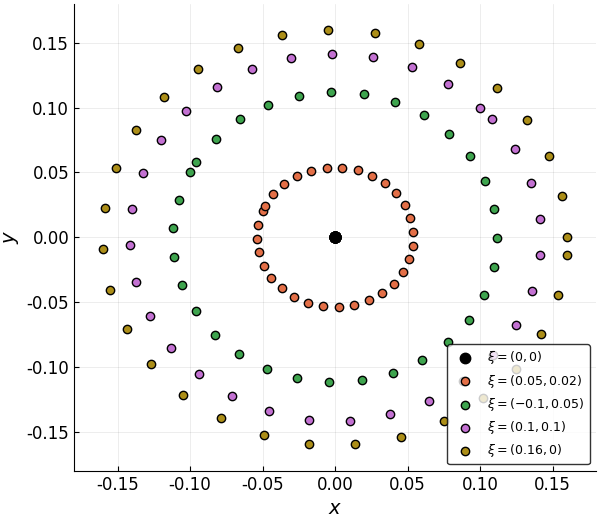
\includegraphics[width=0.8\linewidth]{euler-jt-evaluations-center}
 \caption{Transporte de jets para la ecuación \ref{eq:center} con vecindad inicial $\U_{\xo} = (0,0)^T + \xi$ usando el método de Euler en el intervalo temporal $[0,2\pi]$ en pasos de $h=10^{-4}$. Se evaluó la solución para los distintos $\xi$ marcados en la gráfica, en intervalos de $1000h$.}
 \label{fig:center-evals}
\end{figure}

Notemos que (\ref{eq:center}) corresponde a un sistema hamiltoniano cuyas soluciones en el espacio fase viven en las curvas de nivel dadas por
\begin{equation*}
H(\mathbf{x}) = \frac{1}{2} \left( x_1^2 + x_2^2 \right),
\end{equation*} 
con solución analítica
\begin{align}
 x_1(t) &= x_{01}\cos{(t)} - x_{02}\sin{(t)} \nonumber \\
 x_2(t) &= x_{01}\sin{(t)} + x_{02}\cos{(t)}.
 \label{eq:center_analytical}
\end{align}

En la figura \ref{fig:center_anal_comparison} se muestran distintas comparaciones de la integración numérica contra las soluciones analíticas de (\ref{eq:center_analytical}).

%FIGURA! 
\begin{figure}[h!]
\centering
\begin{subfigure}{0.49\textwidth}
	\centering
	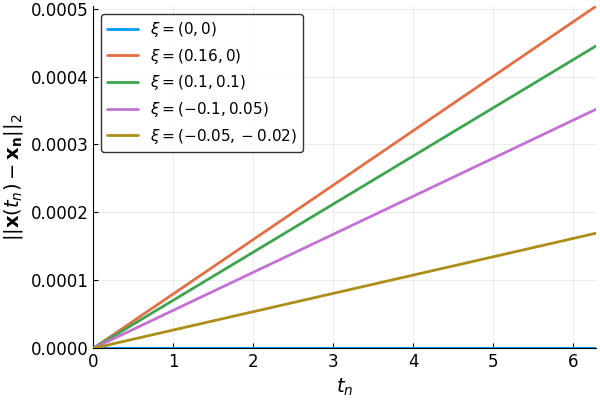
\includegraphics[width = \textwidth]{euler-vs-analytical_center}
	\caption{Norma de la diferencia entre la solución real y evaluaciones de la solución numérica para distintos valores de $\xi$ marcados en la gráfica. Se puede observar un crecimiento lineal del error numérico, lo cual es una de las consecuencias de usar el método de Euler.}
	\label{fig:center-eu_vs_anal}
\end{subfigure}
%
\begin{subfigure}{0.49\textwidth}
	\centering
	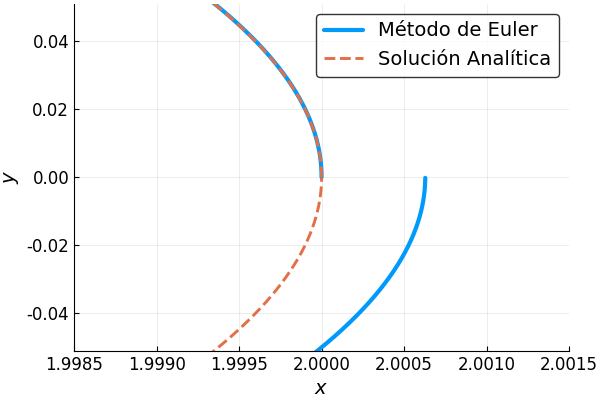
\includegraphics[width = \textwidth]{euler-method_error}
	\caption{Sección del espacio fase donde se observan la solución analítica y la solución numérica para pasos de $h=10^{-4}$ con cóndición inicial $\xo = (2,0)$. \\ \\}
	\label{fig:center_not-closed}
\end{subfigure}
\caption{Diferencias numéricas entre el método de Euler y la solución analítica para \ref{eq:center}}
\label{fig:center_anal_comparison}
\end{figure}


Queda claro que el desarrollo de TJ necesita de un álgebra polinomial para poder evaluar los distintos $P_{j,\xo}(\xi)$ que definen al campo vectorial en cada uno de sus pasos. El problema de evolucionar una vecindad $\U_{\xo}$ dado un sistema dinámico $\dot{\mathbf{x}}(t) = f(t,\mathbf{x}(t))$ se reduce al problema de saber cómo se evalúan distintos polinomios en cada paso de integración, así como la definición computacional de sus operaciones. Hay muchos detalles a considerar en este problema: ¿Qué paso de integración se deberá usar para conseguir la evolución temporal de las soluciones? ¿Cómo medimos el error respecto a la solución real? ¿Existe alguna forma de controlar el error que arrojan el método de integración y la propagación de jets del TJ? ¿Cuál es la complejidad de las operaciones para la aritmética de polinomios? En el apéndice \ref{chap:AlgPoli} se desarrolla el álgebra polinomial y sus operaciones tal como son implementadas en el TJ y se ahonda en esta discusión. En la sección \ref{sec:taylor-metodo} se hace el desarrollo del método de Taylor como integrador computacional adaptativo de sistemas de EDO, y en la sección \ref{sec:ind-dinam} se desarrollan distintos indicadores dinámicos utilizados en el TJ así como sencillos ejemplos ilustrativos para cada uno de ellos.

\section{Método de Taylor}
\label{sec:taylor-metodo}

Como se observa en (\ref{eq:euler}), el método de Euler es la aproximación lineal de $\mathbf{x}(t)$ con $h$ dado. El método de Taylor es la generalización del de Euler en el sentido de que, si $\dotx = f(\mathbf{x}(t),t)$ es una función analítica, entonces $\mathbf{x}(t)$ también lo es y, por tanto, se puede expresar como una serie de potencias convergente 
\begin{equation}
\mathbf{x}(t + h) = \sum_{i=0}^\infty x_i h^i = \sum_{i=0}^\infty \frac{\mathbf{x}^{(i)}(t)}{i!}h^i 
= \sum_{i=0}^M \frac{\mathbf{x}^{(i)}(t)}{i!}h^i + \mathcal{O}(h^{M+1})
\label{eq:anal-exp}
\end{equation}
la expansión de orden $M$ en $h$ donde $x_i$ es la i-ésima derivada normalizada $x_i  := \mathbf{x}^{(i)}(t)/i! $, con $\mathbf{x}^{(i)}(t)$ la i-ésima derivada de $\mathbf{x}(t)$ evaluada en $t$. En el caso que $\mathbf{x}: \mathbb{R} \to \mathbb{R}^d$, entonces $i$ es un índice múltiple tal que $x_i := x_{i_1,\cdots,i_d} \in \mathbb{R}$ e $i :=||\mathbf{i}||_1 = i_1 + \cdots + i_d$, compactando así la notación para dimensiones $d > 1$. El término $\mathcal{O}(h^{M+1}$ corresponde al residuo de la expansión y, en caso de funciones analíticas, son términos de menor corrección a la función expandida dentro del radio de convergencia de ésta. Por esto, el residuo no será tomado en cuenta explícitamente y será considerado como el error del método.

Notemos que comparando ambas expansiones en series de potencias de (\ref{eq:ode}) y notando que $ \frac{d}{dt} \left( \sum_{k=0} a_k t^k \right) = \sum_{k=1} k a_k t^{k-1}$,   
\begin{equation*}
 \dot{\mathbf{x}}(t) \approx \sum_{i=1}^M i x_i t^{i-1} = \sum_{i=0}^M (i+1)x_{i+1} t^i = \sum_{i=0}^M f_i t^i
\end{equation*}

definiendo la relación de recurrencia
\begin{equation}
x_{i+1} = \frac{f_i}{i+1}
\label{eq:rec-rel}
\end{equation}

obteniendo así 
\begin{equation}
\mathbf{x}(t_{n+1}) = \mathbf{x}(t_n) + \sum_{i=1}^M f_i(\mathbf{x}(t_{n+1}),t_n)h^i + \mathcal{O}(h^{M+1})
\label{eq:taylor-rel}
\end{equation}

el \textbf{método de Taylor} para obtener $\mathbf{x}(t) = \flowci$ dado $\xo$.

Una enorme ventaja de (\ref{eq:taylor-rel}) sobre el método de Euler, o cualquier método de integración numérica con paso fijo como varios de los Runge-Kutta, es que se puede acotar el residuo $\mathcal{O}(h^{M+1})$ en términos de $h$, controlando así el error de integración del sistema de EDO para cada paso. Como $f$ y $\mathbf{x}$ son analíticas, entonces su expansión en series de potencias es convergente. De este modo, buscamos que la contribución del último término de la serie sea menor a cierta tolerancia $\epsilon_{Taylor}$, es decir
\begin{equation*}
||x_M||_\infty h^M \leq \epsilon_{Taylor} \implies h = \left( \frac{\epsilon_{Taylor}}{||x_M||_\infty} \right)^{1/M}.
\end{equation*} 

Para el caso de funciones pares o impares, es probable que el último coeficiente de la serie sea identicamente cero y, para evitar indeterminaciones al encontrar $h$, se busca la mínima $h$ entre los dos últimos coeficientes de la expansión de $\mathbf{x}(t+h)$
\begin{equation}
h = \min_{m \in [M-1,M]}{ \left( \frac{\epsilon_{Taylor}}{||x_m||_\infty} \right)^{1/m} }.
\label{eq:stepsize}
\end{equation} 
%% De acuerdo con Simo y la tesis de Dani Perez, esta no es la mejor selección para el paso de integración. De hecho, no pude demosttrar que este paso sea, en efecto, una buena elección. Sin embargo, suena como algo intuitivo ya que la serie es convergente. Ellos, sin embargo, sí acotan de manera formal la contribución del error del residuo... checarlo.

\subsection{Método de Taylor para el transporte de jets}
Para el método que se acaba de desarrollar, cada término satisface que $\mathbf{x}_i \in \mathbb{R}^d$. Sin embargo, en el TJ una vecindad $\U_{\xo}$ se parametriza con el polinomio $P_{0,\xo}(\mathbf{\xi}) \in \pkk{N}{d}$ alrededor de $\xo = \mathbf{x}(t_0)$\footnote{Consultar la sección \ref{sec:pknN} para familiarizarse con esta notación.}. Dado que $P_{0,\xo}(\mathbf{\xi}) = \U_{\xo} = \xo + \mathbf{\xi}$, la relación de recurrencia (\ref{eq:taylor-rel}) puede reescribirse como
\begin{equation}
P_{n+1,\xo}(\xi) = P_{n,\xo}(\xi) + \sum_{i=1}^M f_i(P_{n,\xo}(\xi),t_n)h^i 
\label{eq:jt-rel}
\end{equation}

donde $P_{n,\xo}(\xi) \in \pkk{N}{d} \ \forall \ n$. Así, pueden encontrarse las soluciones $\phi(t_n;t_0,\xo) = \mathbf{x}(t_n)$ con condición inicial $\xo$ y $\phi(t_n;t_0,\U_{\xo}) = P_{n,\xo}(\xi)$ la solución de la vecindad $\U_{\xo}$ al tiempo
$t_n$ del sistema (\ref{eq:ode}) usando (\ref{eq:taylor-rel}) y (\ref{eq:jt-rel}), respectivamente.

Aunque la actualización del método de Taylor para el transporte de jets es bastante directa gracias al desarrollo del álgebra polinomial, hay que prestar atención a cómo obtener el paso de integración $h$ ya que, siguiendo (\ref{eq:stepsize}), debemos tomar $||x_m||_\infty$ y para $x_m \in \pkk{N}{d}$, la p-norma no está definida.

\begin{definicion}
Sea $||\cdot|| : \mathbb{K} \to \mathbb{R}^+$, $P(\mathbf{\xi}) = \sum_{k} a_k \mathbf{\xi}^k \in \mathbb{K} = \pkk{N}{d}$. Se define la \textbf{p-norma} de $P(\xi)$ como
\begin{equation}
 ||P(\mathbf{\xi})||_p := \left( \sum_{k} ||a_k||_p^p \right)^{1/p}
 \label{eq:poly-norm}
\end{equation}  
donde, si $a_k \in \mathbb{R}$, entonces $||a_k||_p = |a_k|$.
\end{definicion}

Así, la elección del paso de integración tiene sentido ahora también para polinomios. Es importante mencionar que la definición de la norma para polinomios en $\pkk{N}{d}$ coincide con la definición estándar de norma. Además, de este modo, el paso de integración $h$ coincide por el utilizado por D. Perez en \cite{P-palau}.

\subsection{Probando el método de Taylor}
\label{sec:benchmark-taylor}

Hemos trabajado, con intención de entender la escencia del transporte de jets, con el método de Euler. Sin embargo, es hora de poner a prueba el método de Taylor desarrollado hace un momento y ver si (\ref{eq:taylor-rel}) y (\ref{eq:jt-rel}) son suficientemente precisos y ver, para (\ref{eq:jt-rel}) en particular, qué tipo de variables e indicadores se pueden obtener para obtener lo mejor del método.

Tomaremos, a manera de ejemplo, un par de \textbf{sistemas hamiltonianos} de la forma
\begin{equation}
 H(\mathbf{p},\mathbf{q}) = \frac{1}{2m}\mathbf{p}^2 + V(\mathbf{q})
 \label{eq:hamiltonian}
\end{equation}
%V = V(p,q) ? 

donde $H: \mathbb{R}^{3N}\times\mathbb{R}^{3N} \to \mathbb{R}$ es el hamiltoniano del sistema y representa la energía, con $N$ la dimensionalidad del espacio. $H$ es una primera integral del sistema
\begin{align}
 \dot{\mathbf{p}} &= -\frac{\partial{H}}{\partial{\mathbf{q}}} \nonumber \\
 \dot{\mathbf{q}} &= \frac{\partial{H}}{\partial{\mathbf{p}}}
\label{eq:ham-rel}
\end{align}

y su primera integral (\ref{eq:hamiltonian}) representa una constante de movimiento que, físicamente, representa la conservación de la energía total.

Así, comprobar los métodos de integración para sistemas conservativos como (\ref{eq:hamiltonian}) será comparar la energía para cada paso temporal dado en relación a la energía inicial, lo cual debería ser constante. 
Dado que conozcamos la solución analítica de algún sistema, se puede comparar dicha solución contra la calculada por los diferentes métodos de integración.

\subsubsection{Oscilador armónico}
\label{sec:oscilador}
Sea un sistema dado por una masa $m$ que, al desplazarlo de su estado de equilibrio por una cantidad $\mathbf{x}$, siente una fuerza restitutiva proporcional a dicho desplazamiento
\begin{equation}
 \mathbf{F}(\mathbf{x}) = m \ddot{\mathbf{x}} = - k\mathbf{x}
 \label{eq:oscilador_force}
\end{equation}
con $[k] = \frac{Kg}{s^2}$  y $k>0$. 

Tomando $\mathbf{v} = \dot{\mathbf{x}}$ se obtienen
\begin{align}
 \dot{\mathbf{x}} &= \frac{k}{m} \mathbf{p} \nonumber \\
 \dot{\mathbf{v}} &= - \frac{k}{m} \mathbf{x}
 \label{eq:oscilador_ode}
\end{align}
las EDO para el \textbf{oscilador armónico}, las cuales son equivalentes, para $\omega^2 := \frac{k}{m} = 1$ y $\mathbf{x} \in \mathbb{R},\ \mathbf{p} \in \mathbb{R}$, a (\ref{eq:center}). 

La primera integral de (\ref{eq:oscilador_ode})
\begin{equation}
 H(\mathbf{p},\mathbf{x}) = \frac{1}{2m}p^2 + \frac{\omega^2}{2} x^2
 \label{eq:oscilador_ham}
\end{equation}
con $p=mv$, cumple con las ecuaciones de (\ref{eq:ham-rel}), una constante de movimiento que representa la energía.

%FIGURA!
\begin{figure}[h!]
 \centering
 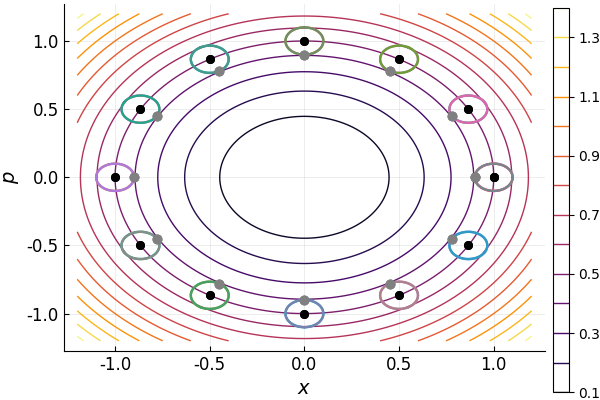
\includegraphics[width=0.8\linewidth]{oscillator_phsp}
 \caption{Espacio fase para el oscilador armónico representado por la ecuación \ref{eq:oscilador_ham}. En negro aparece la solución calculada con el método de Taylor para jets con $\xo = (1,0)^T$, tolerancia $\epsilon_{Taylor} = 10^{-20}$, orden de la expansión $M = 28$ y orden del jet $N=4$. Los jets fueron evaluados para la vecindad parametrizada por $\mathbf{\xi}(\tau) = 0.1\cdot \left( \cos(\tau), \sin(\tau) \right)^T$, $\tau \in [0,1]$, mientras que la solución en gris representa la variación $\xi = (-0.1,0)^T$.}
 \label{fig:oscilador_phsp}
\end{figure}

Así, tenemos que las soluciones analíticas son de la forma 
\begin{align}
 x(t) &= v_{0}\sin{(\omega t)} + x_{0}\cos{(\omega t)} \nonumber \\ 
 v(t) &= v_{0}\omega\cos{(\omega t)} - x_{0}\omega\sin{(\omega t)}. 
 \label{eq:oscilador_analytical}
\end{align}

La figura \ref{fig:oscilador_phsp} presenta al espacio fase del oscilador armónico, junto con una solución calculada con el transporte de jets. En ésta se observa cómo las soluciones evaluadas en una vecindad inicial parametrizada por un círculo están siempre en las líneas de las curvas de nivel del hamiltoniano. Se observa además en la figura la estructura de centros alrededor del único punto singular $(0,0)^T$.

Dada la condición inicial $\xo = (1,0)^T$ y tomando $m = 1 \ Kg$, $k = 1 \frac{Kg}{s^2}$, el oscilador tendrá una energía de $E_0 = H(\xo) = 1$ Joules. En la figura \ref{fig:oscillator_deltas} se pueden ver las variaciones $\delta E(t_n)$ de la energía en cada paso de integración así como la diferencia $\delta \mathbf{x}(t_n)$ de las soluciones de jet calculadas por el método de Taylor evaluadas en diferentes $\xi$s y las soluciones analíticas del oscilador armónico correspondientes al desplazamiento dado por dichas $\xi$s.

%FIGURA!
 \begin{figure}[h!]
\centering
\begin{subfigure}{0.49\textwidth}
	\centering
	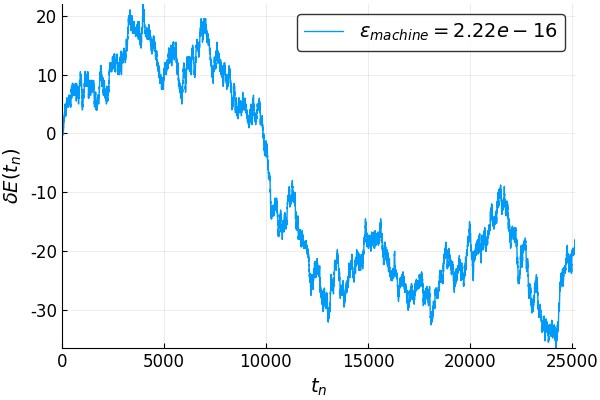
\includegraphics[width = \textwidth]{oscillator_dE}
	\caption{Variación $\delta E(t_n) = \frac{E(t_n)-E_0}{\epsilon_{machine}}$ de la energía respecto a la energía inicial $E_0 = 1$ Joule.\\ \\ }
	\label{fig:oscillator_dE}
\end{subfigure}
%
\begin{subfigure}{0.49\textwidth}
	\centering
	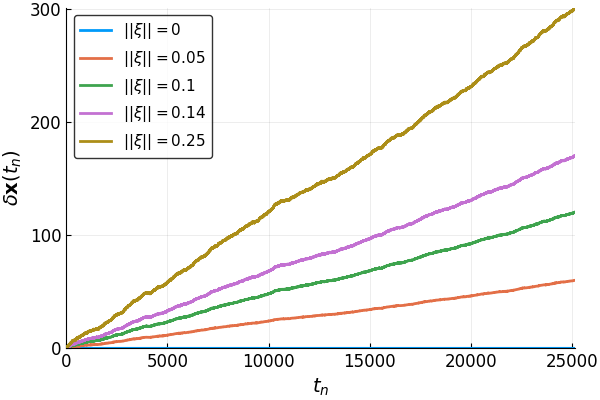
\includegraphics[width = \textwidth]{oscillator_dx}
	\caption{Variación $\delta \mathbf{x}(t) =  \frac{||\mathbf{x}(t_n) - \mathbf{x_n}||_2}{\epsilon_{machine}}$ respecto a la solución analítica (\ref{eq:oscilador_analytical}) para distintos desplazamientos $\xi$ respecto de la condición inicial $\xo$.}
	\label{fig:oscillator_dx}
\end{subfigure}
\caption{Variaciones de energía y trayectoria para el oscilador armónico en cada uno de los pasos temporales de la solución con condición inicial $\xo = (1,0)^T$ y vecindad parametrizada por  $\mathbf{\xi}(\tau) = 0.1\cdot \left( \cos(\tau), \sin(\tau) \right)^T$, $\tau \in [0,1]$. Se utilizó tolerancia $\epsilon_{Taylor} = 10^{-20}$, orden de la expansión $M = 28$ y orden del jet $N=4$.}
\label{fig:oscillator_deltas}
\end{figure}

Es interesante notar que (\ref{eq:oscilador_ode}) es un sistema lineal de ecuaciones y, por tanto, basta con un jet de orden $1$ para obtener la mejor aproximación de las vecindades de $\xo$. De hecho, evaluar $\U_{\xo}$ en $f(\mathbf{x})$ de (\ref{eq:ode}) siempre regresa una cantidad lineal y por tanto, nunca aparecen términos de orden mayor en las variables del sistema de EDO.

\clearpage
\subsubsection{Péndulo simple}
\label{sec:pendulo}
Sea un sistema donde una masa $m$ está anclada al extremo de una varilla de longitud $l$ cuya masa es despreciable. Esta varilla está anclada, a su vez, a un punto inmovil. Así, $m$ se mueve bajo la acción de la gravedad $\mathbf{g}$ como se muestra en la figura \ref{fig:pendulo}, ignorando la resistencia del aire.

%FIGURA! 


La forma más natural de trabajar este problema es en coordenadas polares, en donde la masa $m$ se mueve con una velocidad $v = l\dot{\theta}$ con $l$ constante, es decir $r = l \neq r(t) \implies \dot{r} = \dot{p_r} = 0$. Esta constricción reduce en uno los grados de libertad del sistema, haciendo que éste dependa únicamente de $\theta$. 

Tenemos que 
\begin{align}
 K &= \frac{1}{2}m v^2 = \frac{1}{2} m l^2 \dot{\theta}^2 \nonumber \\
 U &= mgh(\theta) = mgl\left(1 - \cos{\theta} \right)
\end{align}
son la energía cinética y potencial, respectivamente. 

Así, contruimos el lagranjiano del sistema
\begin{equation*}
 \mathcal{L}(\theta,\dot{\theta}) = K - U = \frac{1}{2} m l^2 \dot{\theta}^2 - mgl\left(1 - \cos{\theta} \right).
\end{equation*}
Sabemos, por (\ref{eq:lagr-ham-rel}), que
\begin{equation*}
 \mathbf{p} = \frac{\partial \mathcal{L}}{\partial \mathbf{\dot{q}}} = ml^2\dot{\theta}
\end{equation*}

obteniendo la coordenada conjugada de momento y, así, plantear el hamiltoniano, o energía total del sistema, como
\begin{equation}
 H(p,\theta) = K + U = \frac{p_{\theta}^2}{2ml^2} + mgl\left(1 - \cos{\theta} \right).
\label{eq:pendulo-ham}
\end{equation}
 
Las EDO quedan entonces, por (\ref{eq:ham-rel}), como
\begin{align}
 \dot{\theta} &= \frac{p_{\theta}}{ml^2} \nonumber \\
 \dot{p_{\theta}} &= -mgl\sin{\theta} 
\label{eq:pendulo-ode}
\end{align}

en cuyo dominio $(\theta,p_{\theta}) \in [-\pi,\pi]\times[p_{min},p_{max}] \subset \mathbb{R}^2$ existen tres puntos singulares: $(-\pi,0),(\pi,0), (0,0)$; dos puntos de ``liberación'' y otro de ``relajación'', respectivamente. En la figura \ref{fig:pendulum_pshp} se puede ver una representación del espacio fase donde se exhibe el comportamiento de dichos puntos.

%FIGURA!
\begin{figure}[h!]
 \centering
 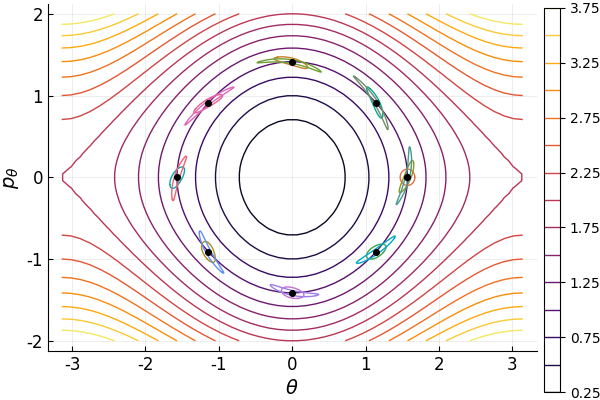
\includegraphics[width=0.8\linewidth]{pendulum_phsp}
 \caption{Espacio fase para el péndulo simple representado por la ecuación \ref{eq:pendulo-ham}. En negro salen puntos de la trayectoria calculada con el método de Taylor para Jets con $\xo = (\frac{\pi}{2},0)^T$, tolerancia $\epsilon_{Taylor} = 10^{-20}$, orden de la expansión $M = 28$ y sus vecindades (jets) evaluadas para $\mathbf{\xi}(\tau) = 0.1\cdot \left( \cos(\tau), \sin(\tau) \right)^T$, $\tau \in [0,1]$.}
\label{fig:pendulum_pshp}
\end{figure}

Si viajamos a un planeta en donde $g = 1 \ \frac{m}{s^2}$ \footnote{A veces, para la física, es más fácil viajar a un planeta donde exista la atracción gravitacional que más nos gusta que hacer a un péndulo girar en la Tierra; qué comodo.} y tomamos una varilla de longitud $l=1$ m y una masa $m=1$ kg,  entonces, para las condiciones iniciales $p_{\theta}(0) = 0 \ N \cdot m$ y $\theta(0) = \pi/2$, la energía total es 
\begin{equation*}
E_0 = H(p_{\theta}(0),\theta (0) ) = 1 \text{ J.}
\end{equation*}

Para dichas condiciones, se puede integrar el transporte de jets y además, evaluarlo para condiciones cercanas y ver cómo se comportan éstas soluciones en el espacio fase, que deben, en teoría, moverse por las curvas de (\ref{eq:pendulo-ham}). Se puede observar de la figura \ref{fig:pendulum_jt} cómo para jets de orden 4, las soluciones se quedan sobre las curvas de nivel del hamiltoniano.

%FIGURA!
\begin{figure}[h!]
\centering
\begin{subfigure}{0.49\textwidth}
	\centering
	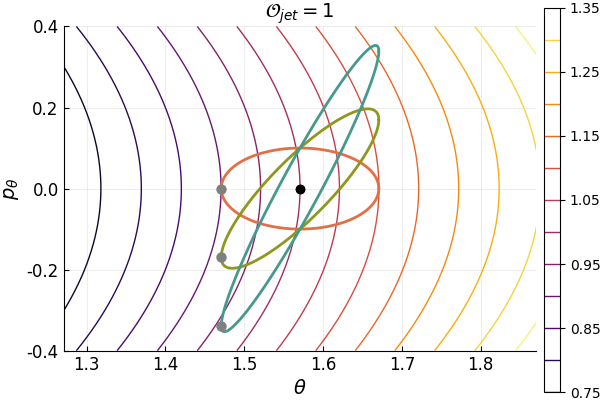
\includegraphics[width = \textwidth]{pendulum_jt_O1}
	\caption{Jet de orden $1$ después de dos periodos desde $\xo$.}
	\label{fig:pendulum_jt_O1}
\end{subfigure}
%
\begin{subfigure}{0.49\textwidth}
	\centering
	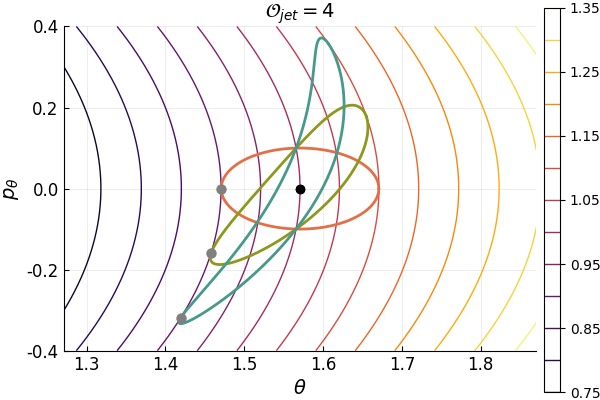
\includegraphics[width = \textwidth]{pendulum_jt_O4}
	\caption{Jet de orden $4$ después de dos periodos desde $\xo$.}
	\label{fig:pendulum_jt_O4}
\end{subfigure}
\caption{Jets de distinto orden para $\U_{\xo}$ parametrizada en un círculo de radio 0.1 $\mathbf{\xi}(\tau) = 0.1\left( \cos(\tau),\sin(\tau) \right)^T$ alrededor de $\xo = (\frac{\pi}{2},0)^T$ en el péndulo simple. Se utilizó tolerancia $\epsilon_{Taylor} = 10^{-20}$ y orden de la expansión $M = 28$.}
\label{fig:pendulum_jt}
\end{figure}

Respecto a las variaciones de energía en el sistema, se ve en la figura \ref{fig:pendulum_dE} cómo $\delta E(t)$ varía alrededor de cero como un movimiento browniano. Éste último se relaciona con los errores de redondeo de puntos flotantes de la máquina y no con el método de Taylor en sí, a diferencia del método de Euler, como se observa en la figura \ref{fig:center_anal_comparison}, donde el error crece de manera lineal. La máxima variación respecto a la energía inicial es de $2.28\times10^{-14}$, lo cual corresponde a $103 \epsilon_{machine}$ (sin redondear).

%FIGURA! 
\begin{figure}[h!]
 \centering
 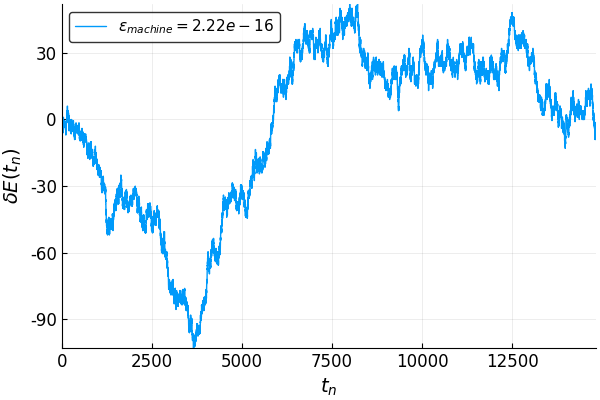
\includegraphics[width=0.8\linewidth]{pendulum_dE}
 \caption{Diferencia $\delta E(t_n) := \frac{E(t_n) - E_0}{\epsilon_{machine}}$ de la energía del péndulo simple con condición inicial $\xo = (\frac{\pi}{2},0)$, tolerancia $\epsilon_{Taylor} = 10^{-20}$ y orden de la expansión $M = 28$.}
 \label{fig:pendulum_dE}
\end{figure}

\clearpage
\subsubsection{Hamiltoniano Artificial}
Inventemos un hamiltoniano que no necesariamente represente un sistema físico. Éste último ejemplo servirá como motivación de la sección siguiente, ya que estaremos analizando las soluciones cerca de una curva límite y se podrá extender un poco la discusión sobre los jets y la necesidad de contruir algunos indicadores dinámicos relevantes. 

Sea 
\begin{equation}
 H(q,p) = qp^2 - \frac{1}{2}q^2
 \label{eq:artificial_ham}
\end{equation}

el hamiltoniano del sistema cuyas curvas de nivel representan las soluciones para la EDO
\begin{align}
 \dot{q} &= 2qp \nonumber \\
 \dot{p} &= -p^2 + q.
 \label{eq:artificial_ode}
\end{align}


Notemos que el sistema anterior tiene un único punto singular $(0,0)^T$ que corresponde a una energía de $H(0,0) = 0$. Con esto, podemos obtener la condición para que las soluciones estén sobre dicho curva límite o separatriz que divide diferentes regiones del espacio. Vemos que si
\begin{equation*}
 H(q,p) = qp^2 - \frac{1}{2}q^2 = 0 \implies p = \pm \sqrt{\frac{q}{2}} 
\end{equation*}

entonces las condiciones iniciales tipo $\xo = \left( q, -\sqrt{\frac{q}{2}} \right)$ vivirán sobre la separatriz. 

%FIGURA!
\begin{figure}[h!]
 \centering
 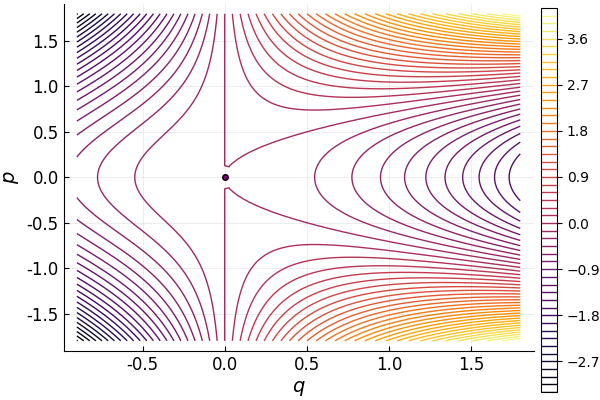
\includegraphics[width= 0.8\linewidth]{artificial_phsp}
 \caption{Espacio fase de \ref{eq:artificial_ode}.}
 \label{fig:artificial_phsp}
\end{figure}

Se muestra en la figura \ref{fig:artificial_phsp} el espacio fase dado por el hamiltoniano del sistema. Notemos que dicha separatriz se puede observar como una especie de parábola horizontal positiva con centro en el punto singular.

%FIGURA!
\begin{figure}[h!]
 \centering
 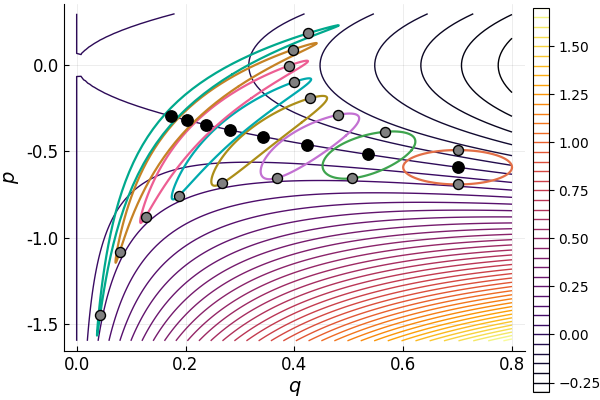
\includegraphics[width= 0.8\linewidth]{artificial_jt_O16}
 \caption{Solución para \ref{eq:artificial_ode}, con condición inicial sobre la separatriz, donde $q0 = 0.7$. Aquí, los jets son de orden $M=16$, en $8$ pasos de integración desde $t_0 = 0$ hasta $t_{max} = 1.7$, con tolerancia $\epsilon_{Taylor} = 10^-{20}$ y orden de la expansión $N=28$. En gris están las soluciones a $\xo + \xi$ sin utilizar TJ.}
 \label{fig:artificial_jt}
\end{figure}

Si tomamos $q_0 = 0.7$ con la condición anterior, y hacemos un transporte de jets alrededor de dicha condición inicial podríamos ver, en teoría, las trayectorias que toman las soluciones cercanas a la curva límite en cada lado de la frontera que ésta impone. En la figura \ref{fig:artificial_jt} se observa la deformación de estos jets conforme pasa el tiempo y, aunque la evolución temporal es un intervalo relativamente corto, es evidente la tendencia que tienen las soluciones cercanas a diverger.

En este problema se vuelve importante muy rápidamente la precisión con la que los jets nos dan soluciones cercanas ya que la deformación de la vecindad inicial $\U_{\xo}$ es muy grande. Por esto, se muestra en la tabla \ref{table:djet_artificial} la diferencia entre evaluar el jet en $\xi = (0,-0.1)^T$ y hacer el método de Taylor convencional partiendo de ese punto. De hecho, se observan en la figura \ref{fig:artificial_jO2_jO16} la evaluación de jets de distinto orden para la misma vecindad inicial alrededor de $\xo$.

%TABLA!
\begin{table}[h!]
\centering
\begin{tabular}{c|ccccc}
\toprule
               & \textbf{$ M = 1 $} & \textbf{$M = 2 $} & \textbf{$ M = 4$} & \textbf{$ M = 8 $} & \textbf{$ M = 16 $} \\ \cmidrule(l){1-6} 
\textbf{$t_0$} & -Inf                       & -Inf                       & -Inf                       & -Inf                       & -Inf                          \\
\textbf{$t_1$} & -2.42                      & -3.97                      & -7.07                      & -13.28                     & -15.95                        \\
\textbf{$t_2$} & -1.92                      & -3.1                       & -5.47                      & -10.22                     & -15.95                        \\
\textbf{$t_3$} & -1.54                      & -2.48                      & -4.37                      & -8.15                      & -15.91                        \\
\textbf{$t_4$} & -1.21                      & -1.96                      & -3.47                      & -6.49                      & -12.53                        \\
\textbf{$t_5$} & -0.91                      & -1.49                      & -2.68                      & -5.05                      & -9.79                         \\
\textbf{$t_6$} & -0.61                      & -1.05                      & -1.95                      & -3.74                      & -7.34                         \\
\textbf{$t_7$} & -0.29                      & -0.6                       & -1.24                      & -2.52                      & -5.08                         \\ \bottomrule 
\end{tabular}
\caption{Diferencia logarítmica de $\delta \mathbf{x} = || \phi(t_i,t_0,\xo + (0,-0,1)^T) - P_{i,\xo}((0,-0.1)^T) ||$ para polinomios $P_{i,\xo}(\xi)$ de distinto orden $M$ en $\xi$.}
\label{table:djet_artificial}
\end{table}

%FIGURA!
\begin{figure}[h!]
 \centering
 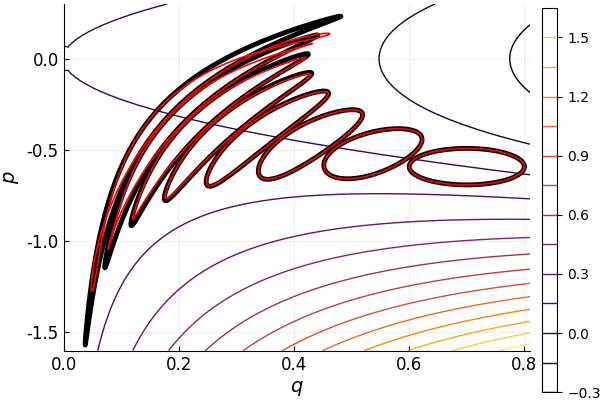
\includegraphics[width= 0.7\linewidth]{artificial_jO2_jO16}
 \caption{Diferencia gráfica entre un jet de orden $M=2$ contra uno de orden $M=16$ para las mismas condiciones.}
 \label{fig:artificial_jO2_jO16}
\end{figure}

Recordemos que como \ref{eq:artificial_ode} es un sistema de EDO hamiltoniano entonces deberá conservar la energía. En la figura \ref{fig:artificial_dE} se observa la variación de la energía para cada paso temporal con el jet evaluado en $\xi = (0,\pm 0.1)^T$, así como en $\xo$, i.e., para el método de Taylor sin jets. Notemos cómo al principio (figura \ref{fig:}) la energía sí se conserva, i.e, las evaluaciones del TJ se mantienen sobre las superficies de nivel del hamiltoniano, sin embargo, cuando la vecindad se empieza a deformar más, la energía empieza a variar más respecto a la de su condición inicial. Notemos que aunque esta variación es de $\approx 10^8 \epsilon_{machine}$, el error en la energía es en la octava cifra significativa, dado que $\epsilon_{machine} = 2.22\times 10^{-16}$.

%FIGURA!
\begin{figure}[h!]
 \centering
 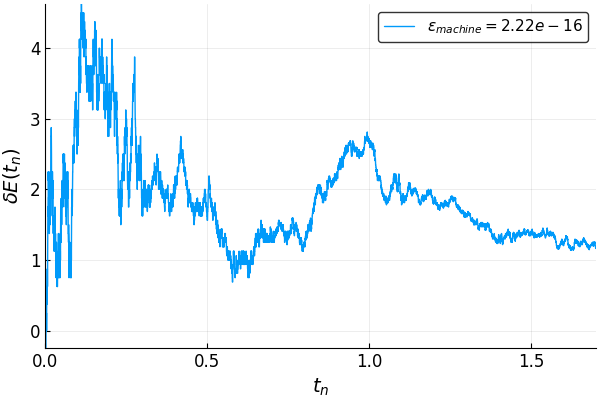
\includegraphics[width=0.7\linewidth]{artificial_dE}
 \caption{Diferencia en energía $\delta E(t_n) = \frac{1}{\epsilon_{machine}} \left( H(\mathbf{x}(t_n)) - H(\xo) \right)$ para el sistema \ref{eq:artificial_ode} sin transporte de jets, con tolerancia $\epsilon_{Taylor} = 10^{-20}$, orden de expansión $N = 28$ y $8000$ pasos temporales de $t_0 = 0$ a $t_{max} = 1.7$.}
 \label{fig:artificial_dE}
\end{figure}

%FIGURA!
\begin{figure}[h!]
\centering
\begin{subfigure}{0.49\textwidth}
	\centering
	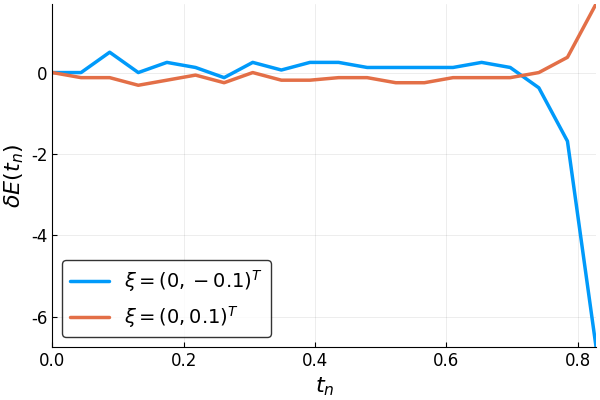
\includegraphics[width = \textwidth]{artificial_dEjets_half}
	\caption{Diferencias de energía $\delta E$ respecto a la energía inicial en la primera mitad de la integración.}
	\label{fig:artificial_dEjets_half}
\end{subfigure}
%
\begin{subfigure}{0.49\textwidth}
	\centering
	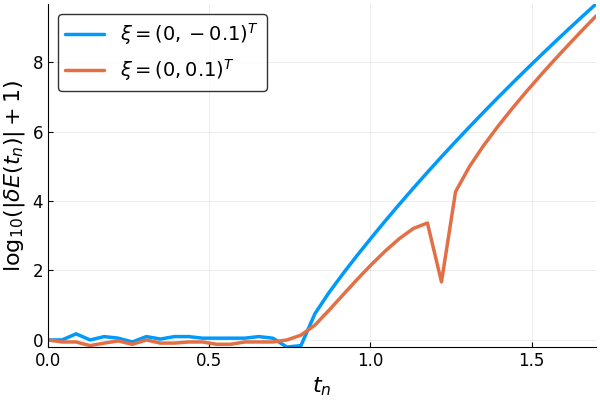
\includegraphics[width = \textwidth]{artificial_dEjets_all}
	\caption{Logaritmo de las diferencias de energía $\delta E$ respecto a la energía inicial en toda la integración.}
	\label{fig:artificial_dEjets_all}
\end{subfigure}
\caption{Diferencia en energía $\delta E(t_n) = \frac{1}{\epsilon_{machine}} \left( H(\mathbf{x}(t_n)) - H(\xo) \right)$ para el sistema \ref{eq:artificial_ode} con jets de orden $M=16$ evaluados en $\xi$. Se utilizó tolerancia $\epsilon_{Taylor} = 10^{-20}$, orden de expansión $N = 28$ y $40$ pasos temporales de $t_0 = 0$ a $t_{max} = 1.7$.}
\label{fig:pendulum_jt}
\end{figure}


Todos los ejemplos construidos en la última sección han sido evaluados en una vecindad con un radio de $r = 0.1$ alrededor de $\xo$. Sin embargo, nada asegura que ésta sea una buena elección para dicha vecindad. Estudiar cuál es el tamaño máximo que una vecindad puede tomar para que los jets arrojen soluciones precisas se vuelve una pregunta natural al ver las gráficas y tablas de éstos ejemplos. Por otro lado, hemos visto en éste último ejemplo cómo una vecindad inicial puede deformarse bastante rápido cerca de una curva límite cuando en el oscilador armónico, en cambio, no se deforma nada. Establecer una métrica de deformación se vuelve, también, una forma de análisis del estudio de vecindades de alguna condición $\xo$ dada para algún sistema de ecuaciones diferenciales a trabajar. En el caso del péndulo simple, se observa cómo después de cada periodo de oscilación, el jet se deforma de manera tal que las soluciones cercanas no cruzan la condición inicial al mismo tiempo que $\xo$; esto se puede estudiar si pintamos una sección transversal a las soluciones del péndulo que pase por $xo$ y observamos en qué tiempo cruzan las vecindades esta sección. El uso de jets motiva a hacer varios indicadores sobre la dinámica de las ecuaciones son obtener explícitamente la solución. Es importante notar que no siempre se tendrá un hamiltoniano explicito para comparar las soluciones con sus curvas de nivel, así que estos indicadores servirán para darnos información sobre el espacio fase sin conocerlo del todo. 

\section{Indicadores dinámicos de campos vectoriales con base en el transporte de jet}
\label{sec:ind-dinam}

%choro

\subsection{Tamaño máximo de las vecindades}


% Para que de nuevo haya salto de linea. (buscar Dutch style)
\setlength{\parskip}{1.3ex plus 0.2ex minus 0.2ex}

\chapter{Resultados} 
\label{chap:Resultados}
\input{Chapters/03_resultados}

% Para que de nuevo haya salto de linea. (buscar Dutch style)
\setlength{\parskip}{1.3ex plus 0.2ex minus 0.2ex}

\chapter{Conclusiones} 
\label{chap:Conclusiones}
\input{Chapters/04_conclusiones}

 
% Para que de nuevo haya salto de linea. (buscar Dutch style)
\setlength{\parskip}{1.3ex plus 0.2ex minus 0.2ex}





 
%%%%%%%%%%%%%%%%%   APÉNDICES   %%%%%%%%%%%%%%%%%
\cleardoublepage 
\phantomsection  %para el anclado este en la pagina correcta
\addcontentsline{toc}{chapter}{Apéndices}
\chaptermark{Apéndices} %cambia el encabezado
\appendix

% Reajuste de los encabezados para que diga Apendice 
\pagestyle{fancy}
\fancyhead[LO]{\leftmark}
\fancyhead[RE]{\emph{Apéndice \thechapter}}
\renewcommand{\headrulewidth}{0.5pt}

\chapter{El código}
\label{chap:Codigo}
\input{Chapters/codigo}

\chapter{Álgebra Polinomial}
\label{chap:AlgPoli}
%% ************************************************************************
%% &&&&&&&&&&&&&&&&   01. ÁLGEBRA POLINOMIAL  &&&&&&&&&&&&&&&&&&&&&&&&&&&&&
\section{Construcción del Álgebra}

Como se menciona en la introducción, para poder hacer el transporte alrededor de todo una vecindad $\mathcal{U}$ de manera numérica es importante diseñar un integrador de las ecuaciones que cargue toda la información de $\mathcal{U}$ para cada paso temporal. Esto se puede lograr si en lugar de hacer evolucionar al integrador con escalares en $\mathbb{R}$ o $\mathbb{C}$ se hace con un polinomio con centro en la condición inicial $\bm{x_0} := \bm{x}(t=0)$ , de modo que para cada paso se tiene un nuevo polinomio que representa la evolución del polinomio en el paso anterior, el cual se puede sustituir por reales y obtener así puntos de la vecindad de $\bm{x_0}$. \\

Dicho lo anterior, es necesario desarrollar un álgebra polinomial que denotaremos como $\algpol$ donde $\pk$ es el conjunto de \textbf{polinomios de orden $n$ con coeficientes en el campo $\mathbb{K}$} tal que, si  $P(x) \in \pk$, éste se define como
$$P = P(x) := \polk{p_k} $$
con $P: \mathbb{C} \to \mathbb{K}$ una función analítica y $p_k \in \mathbb{K} \  \forall i \in [0,n]$.

%		- It may be necessary to analize how different independet variables imply that A(x) != A(b).


Inspirado en la aritmética usual en $\mathbb{C}$ o $\mathbb{R}$, podemos definir $(+,\cdot)$ para $\algpol$ de la siguiente manera:

Sean $A,B \in \pk$ con $A = \polk{a_k}$ y $B = \polk{b_k} \ a_k,b_k \in \mathbb{K} \ \forall k \in [0,n]$, entonces, para la suma, notemos que
\begin{align*}
\polk{a_k} + \polk{b_k} =& a_0 + a_1 x + \cdots a_n x^n + b_0 + b_1 x + \cdots + b_n x^n \\
=& (a_0 + b_0) + (a_1 + b_1) x + \cdots + (a_n + b_n)x^n = \polk{(a_n + b_n)} 
\end{align*}
así, se define \textbf{$+$}  en $\pk$ como
\begin{equation}
A + B = \polk{(a_k + b_k)}.
\label{eq: polsum}
\end{equation}

Para el producto, notemos que
\begin{align*}
\polk{a_k}\cdot\polk{b_k} =& (a_0 + a_1 x + \cdots + a_n x^n)\cdot(b_0 + b_1 x + \cdots + b_n x^n) \\
=& (a_0b_0) + (a_1b_0 + a_0b_1) x + (a_2b_0 + a_1b_1 + a_0b_2) x^2 + \cdots + \\
+& \sum_{j=0}^n a_{n-j}b_j x^n + \mathcal{O}(x^{n+1}) = \polk{ \polj{a_{k-j}b_j } }
\end{align*}

así, se define \textbf{$\cdot$}  en $\pk$ como

\begin{equation}
A \cdot B = \polk{\sum_{j=0}^k a_{k-j}b_j}.
\label{eq: polprod}
\end{equation}
Aún cuando las operaciones están definidas inspiradas en la aritmética de los números, $\mathbb{K}$ puede ser cualquier campo arbitrario.

\begin{proposicion}
Para $\mathbb{K} = \mathbb{R}$ o $\mathbb{C}$, $\algpol$ forma un campo.
\end{proposicion}

\begin{proof}
Basta probar las nueve propiedades de campo con las operaciones de \ref{eq: polsum} y \ref{eq: polprod}.
Sean $A$, $B$ y $C \in \pk$
\begin{enumerate}

 \item $ A + B = B + A $
 \begin{proof}
  \begin{align*}
   A + B =& \polk{a_k} + \polk{b_k}  = \polk{(a_k + b_k)} \\ 
   =& \polk{(b_k + a_k)} = \polk{b_k} +     \polk{a_k} = B + A
  \end{align*}
 \end{proof}
 
 \item A + (B+C) = (A+B) + C
 \begin{proof}
  \begin{align*}
   A + (B+C) =& \polk{a} + \polk{(b_k+c_k)} = \polk{(a_k + (b_k + c_k))} \\
   =&  \polk{((a_k + b_k) + c_k)} = \polk{(a_k+b_k)} + \polk{c_k} \\
   =& (A+B) + C 
  \end{align*}
 \end{proof}
 
 \item $\exists \  \bm{0} \in \pk \text{ tal que }  \bm{0} + A = A $
 \begin{proof}
 Sea $\mathbb{0} = \bm{0}(x) = \polk{\sigma_k}$ donde $\sigma_k = 0 \ \forall k \in [0,n]$, así 
  \begin{align*}
  \bm{0} + A = \polk{(\sigma_k + a_k)} = \polk{(0 + a_k)} = \polk{a_k} = A
  \end{align*}
 \end{proof}
 
 \item $\exists \ {-A} \in\pk  \text{ tal que } A + (-A) = 0 $
 \begin{proof}
 Sea $-A = -A(x) = \polk{\mathrm{a}_k}$ donde $\mathrm{a}_k = -a_k \ \forall k \in [0,n]$, así
  \begin{align*}
   A + (-A) = \polk{(a_k + \mathrm{a}_k)} = \polk{(a_k + (-a_k))} = \polk{0} = \bm{0}
  \end{align*}
 \end{proof}
 
 \item $ A\cdot B = B\cdot A $
 \begin{proof}
 Hay que probar, básicamente, que $\sum_{j=0}^k{a_{k-j}b_j} = \sum_{j=0}^k{b_{k-j}a_j}$:
  \begin{align*} 
   \sum_{j=0}^k{a_{k-j}b_j} =& \sum_{i=0}^k{a_ib_{k-i}} \text{ con } i = k - j \\
   =& \sum_{i=0}^k{ b_{k-i}a_i } = \sum_{j=0}^k { b_{k-j}a_j }
  \end{align*}
  $\therefore A\cdot B = B\cdot A$.
 \end{proof}
 
 \item $ (A \cdot B) \cdot C = A \cdot (B \cdot C) $
 \begin{proof}
 Por un lado
  \begin{align*}
  A \cdot (B \cdot C) =& \polk{a_k}\ \polk{ \polj{b_{k-j}c_j} } = \polk{\big(  \sum_{j=0}^ka_{k-j}\sum_{i=0}^jb_{j-i}c_i \big)} \\
  =& \polk{\big(  \sum_{r+j=k}a_r\sum_{p+i=j}b_pc_i \big)} = \polk{\big(  \sum_{r+j=k}\sum_{p+i=j}a_rb_pc_i \big)} \\
  =& \polk{\big(  \sum_{r+p+i=k}a_rb_pc_i \big)} 
  \end{align*}
  por otro
    \begin{align*}
  (A \cdot B) \cdot C =& \polk{ \polj{a_{k-j}b_j} }\ \polk{c_k} = \polk{\big( \sum_{i=0}^ja_{j-i}b_i  \sum_{j=0}^kc_{k-j} \big)} \\
  =& \polk{\big(  \sum_{r+j=k}(\sum_{p+i=r}a_pb_i) c_j \big)} = \polk{\big(  \sum_{r+j=k}\sum_{p+i=r}a_pb_ic_j \big)} \\
  =& \polk{\big(  \sum_{p+i+j=k}a_pb_ic_j \big)} 
  \end{align*}
  
  Basta ver que, por un cambio de nombre de índices $p \to r$, $i \to p$, $j \to i$,
  \begin{align*}
   \sum_{p+i+j=k}a_pb_ic_j = \sum_{r+p+i=k}a_rb_pc_i
  \end{align*}   
  $\therefore (A \cdot B) \cdot C = A \cdot (B \cdot C)$.
 \end{proof}
 
 \item $\exists \ \textbf{1} \in \pk \text{ tal que } \textbf{1}\cdot A = A $
 \begin{proof}
 Sea $ \textbf{1} = \textbf{1}(x) = \polk{\omega_k}$ donde $\omega_k = 0 \ \forall k > 0$ y $\omega_0 = 1$, así:
 \begin{align*}
  \textbf{1} \cdot A = \polk{ \polj{a_{k-j}\omega_j} } = \polk{ a_{k-0} \cdot 1 } 
  =& \polk{a_k} = A 
 \end{align*}
 \end{proof}
 
 \item $\exists \  A^{-1} \in \pk \text{ tal que } A \cdot A^{-1} = \textbf{1} \ \forall A \text{ con } a_o \neq 0 $
 \begin{proof}
 Sea $A^{-1} = A^{-1}(x) = \polk{\alpha_k}$; con 
 \end{proof}
 \begin{align*}
  A \cdot A^{-1} = \polk{ \polj{a_{k-j}\alpha_j} } \text{ así, buscando} \\
  \sum_{j=0}^k a_{k-j} \alpha_j = 0 \ \forall \ k>0 \text{ y }  \alpha_0 = \frac{1}{a_0}  
 \end{align*}
 podemos llegar a una fórmula recursiva para $\alpha_k$
 \begin{align*}
 \alpha_k = -\frac{1}{a_0} \sum_{j=0}^{k-1}a_{k-j}\alpha_j.
 \end{align*}
 Así, por construcción, se obtiene que $ A \cdot A^{-1} = \textbf{1} $.
 \item $ A \cdot (B+C) = A \cdot B + A \cdot C $
 \begin{proof}
  \begin{align*}
  A \cdot (B+C) =& \polk{a_k} \big(\polk{(b_k + c_k)} \big) = \polk{\polj{a_{k-j}(b_j+c_j)}} \\
  =& \polk{ \big( \polj{a_{k-j}b_j} \polj{a_{k-j}c_j} \big) } = A \cdot B + A \cdot C
  \end{align*}   
 \end{proof}
 
\end{enumerate}
Así, quedan demostradas todas las propiedades de campo. \qed
\end{proof}

Visto eso, es práctico definir otras operaciones que serán de ayuda al trabajar con elementos de $\pk$. Serán la potencia, la composición y la derivada nuestros ` caballos de batalla '' para el desarrollo de casi cualquier función existente en la aritmética usual.

Sea $A = A(x) = \polk{a_k} \in \pk$. Si $m \in \mathbb{N}$,
\begin{align*}
 A^m =& \big(\polk{a_k}\big)^m = \polk{a_k}\polk{a_k}\big(\polk{a_k}\big)^{m-2} \\
 =& \polk{\polj{a_{k-j}a_j}}\polk{a_k}\big(\polk{a_k}\big)^{m-3} = \polk{{^1\alpha_k}}\polk{a_k}\big(\polk{a_k}\big)^{l-3} \\
 =& \cdots = \polk{{^m\alpha_k}} \\
 &\text{con } {^1\alpha_k} = \polj{a_{k-j}a_j} \text{ y } {^m\alpha_k} = \polj{{^{m-1}\alpha_k}a_j} \\
\end{align*}
y , aunque no queda clara la forma explícita de ${^m\alpha_k}$, se muestra que la \textbf{potencia} está bien definida y que $A^m \in \pk$.


Con esto último, y sea $B = \polk{b_k} \in \pk$, se puede desarrollar
\begin{align*}
 B(A(x)) = B(A) =& \sum_{k=0}^n b_k \big( \sum_{j=0}^n a_j x^j  \big)^k = \polk{b_k} \sum_{j=0}^n {^k\alpha_j x^j} =\polk{ \polj{b_{k-j} {^k\alpha_j} } }
 \end{align*}
que corresponde a la \textbf{composición} de $A$ en $B$, la cual está bien definida y pertenece a $\pk$.

Inspirados en la derivada usual de polinomios de orden $n$ $P: \mathbb{C} \to \mathbb{C}$, tenemos que

\begin{align*}
 \frac{dP(x)}{dx} := P'(x) = P' = \sum_{k=0}^n{k p_k x^{k-1}} = \polk{(k+1)p_{k+1}} 
\end{align*}

así, se define la \textbf{derivada} de $A$ como

\begin{align}
 A' = \polk{(k+1)a_{k+1}}
 \label{eq:polderiv}
\end{align}

con $a_{n+1} := 0 \in \mathbb{K}$ tal que $A' \in \pk$. De la definición usual de derivada podemos ver cómo la \textbf{regla de la cadena} también tiene sentido en este campo, ya que 
\begin{align*}
 { A(B(x))}' :=& \lim_{x \to a}\frac{A(B(x)) - A(B(a))}{x-a} = \lim_{x \to a} \frac{A(B(x)) - A(B(a))}{B(x)-B(a)}\frac{B(x) - B(a)}{x-a}  \\
 =& \lim_{x \to a} \frac{A(B(x)) - A(B(a))}{B(x)-B(a)} \lim_{x \to a} \frac{B(x) - B(a)}{x-a} = A(B(x))'B(x)'
\end{align*}

lo cual se puede traducir a 
\begin{align*}
\lim_{x \to a} \big( A(B(x)) + \ - A(B(a)) \big) \cdot \big( (B(x) + \ -B(a) \big)^{-1} \cdot \lim_{x \to a} \big( (B(x) + \ -B(a) \big) \cdot \big( \textbf{1(x)} + \ -\textbf{1(a)} \big)    
\end{align*}
con las operaciones definidas hasta ahora.

%		- See "chain rule" technical details. Maybe only mention taht is has sense for polynomial functions and later on prove that it is indeed true.
%		- Define (/,-,sin,cos,exp,log,pow). This should be expanded when needed in the thesis only.

Aún cuando ya tenemos las operaciones básicas del álgebra definidas, va a ser de gran practicidad extender otras operaciones útiles para el transporte de $\mathbb{U}$ para el campo vectorial que estemos estudiando.

Se define la \textbf{resta $-$} como
\begin{equation}
 A - B := A + (-B).
 \label{eq:polisub}
\end{equation}


Para la división, sea $D(x) \in \pk$, tal que  $B \cdot D = A $,  entonces 
\begin{align*}
 & \polk{ \polj{b_{k-j} d_j} } = \polk{ a_k } \implies \polk{ a_k - \polj{b_{k-j} d_j} } = 0 \\ 
 &\implies a_k - ( \sum_{j=0}^{k-1}a_{k-j} d_j + b_0 d_k ) = 0 \\
 & \therefore d_k = \frac{1}{b_0} \big( a_k - \sum_{j=0}^{k-1} b_{k-j} d_j \big)  
\end{align*}

Se define la \textbf{división} como
\begin{equation}
 D = A/B \text{ con } d_k = \frac{1}{b_0} \big( a_k - \sum_{j=0}^{k-1} b_{k-j} d_j \big)
 \label{eq:polidiv}
\end{equation}

Con el mismo espíritu, inspirados por el artículo de Haro ~\cite{Haro2009} podemos definir más relaciones de recurrencia para otras operaciones entre polinomios.

%		- Maybe I can make just a few and then cite "Haro"... in the spirit of Haro, other functions will be defined as ---

Fantástico, $^nP_{\mathbb{C}}$ y $^nP_{\mathbb{R}}$ son campos y tenemos ya varias operaciones definidas sobre $\pk$, pero la motivación del desarrollo de este álgebra es hacer polinomios de una variable (que representen al tiempo) cuyos coeficientes sean polinomios de varias variables (que representen al espacio fase de $\dot{x} = f(x(t))$), cuyos coeficientes sean elementos de $\mathbb{C}$ o $\mathbb{R}$. Es decir, nos gustaría trabajar con polinomios cuyos coeficientes sean polinomios, cuyos coeficientes sean, finalmente, números.
Sea  $\pk$ con $\mathbb{K} = {{^{n}P_{\mathbb{C}}}}$, entonces, con $P(x) \in \pk$ y $P_k(y) = \sum_{j=0}^n a_{j,k}y^j \in \mathbb{K} \forall k \in [1,n]$

\begin{equation}
 P(x) =  \polk{P_k(y)} = \polk{\left( \sum_{j=0}^n a_{j,k} y^j \right)} := \sum_{k+j=0}^n a_{j,k} y^j x^k = P(\mathbf{x}).
\label{eq:pkn2}
\end{equation}

Con la definición planteada en la última igualdad de \ref{eq:pkn2} se observa cómo el polinomio $P(x)$ cuyos coeficientes son los polinomios $P_k(y)$ es equivalente a un polinomio de dos variables que vive en un espacio que denominaremos, por construcción, $\pkn{2}$. Se tuvo que imponer la condición de que en el último conjunto de términos $i+j = n$ así $P(x)$  pueda pertenecer, en efecto, a un espacio de polinomios de orden $n$.

Inductivamente, se puede construir el espacio $\pkn{N}$ tomando
\begin{align}
 P(x_1) = \sum_{k_{1}=0}^n\sum_{k_2=0}^n\cdots\sum_{k_N=0}^n a_{k_{1},k_{2},\cdots,k_{N}}x_N^{k_{N}}x_{N-1}^{k_{N-1}} \cdots x_1^{k_{1}} := \sum_{||\mathbf{k}||_{1}=0}^n a_{\mathbf{k}}\mathbf{x}^{\mathbf{k}}
\label{eq:pknN}
\end{align}

con $\mathbf{k} = (k_1,\cdots,k_N)$, $||\mathbf{k}||_1 = k_1+k_2+\cdots+k_N$ la 1-norma de $\mathbf{k}$ y $\mathbf{x} = (x_1,\cdots,x_N)^T$. Así, quedan bien definidos los polinómios de orden $n$ en $N$ variables con coeficientes en $\mathbb{C}$ (y en $\mathbb{R}$, naturalmente) en el espacio $\pkn{N}$ como la suma de polinomios homogeneos desde orden $0$ hasta $N$.

%%Con esto contruido, se puede hablar de los Taylors anidados de manera muy natural, que nacen de NO truncar a orden n el espacio; notar que los espacios $\pk$ con $\mathbb{K} = {{^{n}P_{\mathbb{C}}}}$ y $\pkn{2}$ son escencialmente distintos ya que no son del mismo orden...

En el caso del transporte de jets se trabaja en el espacio ${^{m}P_{\mathbb{K}}}$, $\mathbb{K} = \pkn{N}$, con $m$ el orden de la expansión temporal del método de Taylor y $n$ el orden de la expansión polinomial de $f$ en \ref{eq:ode} evaluada en $\U_{\xo}$. 

\section{Integrador de Taylor}

Ahora que ya están definidas todas las operaciones de polinomios es buen momento para desarrollar al integrador numérico que nos permitirá hacer el transporte mencionadas en la introducción.

La idea básica de un integrador es que, dado un sistema de $n$ ecuaciones diferenciales

\begin{align}
 \dot{\bm{x}(t)} := \frac{dx_i(t)}{dt} = f_i(t;\bm{x}(t)) \ \forall i \in [1,n]
 \label{eq: eqdif}
\end{align}

se encuentre un método que evolucione de la mejor manera posible dada una condición inicial $\bm{x_0}$ o, en nuestro caso, una \textit{bola} inicial {$B_{\bm{x_0}}$} a cada paso del parámetro $t$ (tiempo) que rige la ecuación. El tema con un integrador numérico es que éste pretende evaluar todos los tiempos contenidos entre la condición inicial y la final y, como ninguna máquina ha sido capaz de evaluar una cantidad continua en un intervalo, es necesario discretizar al parámetro que hace que nuestras ecuaciones evolucionen.

Una forma muy intuitiva de abordar este problema es con el método de Euler, que parte de la definición usual de derivada. Tomemos el caso de una función analítica $f: \mathbb{R}  \to \mathbb{R}$, entonces

\begin{align}
 \dot{f}(t) := \frac{df(t)}{dt} = \lim_{h\to 0} \frac{ f(t+h) - f(t) }{h}
 \label{eq: deriv}
\end{align}

Si tomamos el límite $h \to 0$ de una manera menos rigurosa y lo tratamos simplemente como un \textit{incremento muy pequeño}, podemos tener una aproximación razonablemente buena de la derivada, donde

\begin{align*}
\dot{f}(t) := \frac{ f(t+h) - f(t) }{h} + R(t;h)
\end{align*}

donde $R$ es un residuo que depende de $h$ y decrece con ella. Si esto lo aplicamos a \ref{eq: eqdif} cuando $\textbf{x} \in \bm{R}^n$, entonces

\begin{align}
 \bm{f}(\bm{x}(t)) = \frac{d\bm{x}(t)}{dt} =& \frac{ \bm{x}(t+h) - \bm{x}(t) }{h}+ \bm{R}(h)\\
 \implies \bm{x}(t+h) =& \bm{x}(t) + h\cdot \bm{f}(\bm{x}(t)) - \bm{R}(t;h)
 \label{eq: poli1g}
\end{align}
\begin{align}
 \to \ & x_{i_{n+1}} = x_{i_n} + h\cdot f_n - R_{1_i}(h) \ \forall i \in [1,n]
 \label{eq: euler}
\end{align}

que plantea una relación de recurrencia, conocida como el \textbf{método de Euler}. Aún cuando esta relación no es tan poderosa y no es, definitivamente, la que se usará en los cálculos desarrollados en la presente tesis, es interesante notar que \ref{eq: euler} es ahora un \textit{mapeo} que resuelve la ecuación diferencial de manera discreta, con un \textit{salto temporal} de tamaño $h$ y un error o residuo $R_{1_i}(h)$ y esto se conservará para cualquier método empleado.\\

En lugar de tomar una condición inicial $\bm{x_0}$, nos interesa tomar el polinomio

\begin{align*}
 \ball{0} = \bm{x}_0 + \bm{\mu}
\end{align*}

que representa a la condición inicial $\bm{x_0}$ más alguna perturbación definida  por el vector de polinomios $\bm{\mu}$, similar a como se hace en \cite{Perez2015}. Con las operaciones definidas en la sección anterior se puede desarrollar la relación de recurrencia \ref{eq: euler} tal que 

\begin{align*}
 \bm{x_1} =&  \ball{1} =  \ball{0} + h\cdot\bm{f}( \ball{0}) \\ 
 =& \big( \bm{x_0} + h\cdot \bm{f}(\bm{x_0}) \big) +  \big( \bm{\mu} + h\cdot \bm{f}(\bm{\mu}) \big) + \bm{R}_1(h)
\end{align*}

que representa el primer paso temporal del método de Euler pero con la condición inicial $\ball{0}$, que hace uso del álgebra de polinomios desarrollado en la sección anterior. Es interesante notar que el tranporte de bolas si puede hacer con cualquier integrador numérico. Generalizar este método es simplemente extender la o las funciones del sistema de ecuaciones diferenciales asociadas hasta algún orden $N$, donde si $f_i$ en \ref{eq: eqdif} es analítica $\forall i$, entonces 

\begin{align}
 \bm{x}(t+h) = \bm{x}(t) + \bm{x}^{\prime}(t)h + \frac{1}{2!}\bm{x}^{\prime\prime}(t)h^2 + ... + \frac{1}{n!}\bm{x}^{(n)}(t)h^n + \bm{R}^{n+1}(h)
\end{align}
que, por \ref{eq: eqdif},
\begin{align}
 \bm{x}(t+h) =& \bm{x}(t) + \bm{f}(t;\bm{x}(t))h + \frac{1}{2!}\bm{f}^\prime(t;\bm{x}(t))h^2 \\ 
 +& ... + \frac{1}{n!}\bm{f}^{(n-1)}(t;\bm{x}(t))h^n + \bm{R}^{n+1}(h)
 \label{eq: taylorint}
\end{align}

definiendo así la relación de recurrencia del \textbf{método de Taylor}. Notemos que \ref{eq: taylorint} también puede ser evaluada por $\ball{0}$, siempre y cuando estén definidas las operaciones para $\bm{f}$ y todas sus derivadas en el intervalo de interés.

Hay que prestar especial atención al error que pueda tener la ecuación en cada paso temporal, ya que éste determinará qué tan preciso es el método y qué tan fiable es la solución que obtenemos al integrar para un intervalo de tiempo dado. Se busca encontrar cómo varía el error en función del orden del polinomio escogido y el tamaño del paso de integración $h$.

En el apéndice \textit{Taylor series methods of integration} de Simó (2001) ~\cite{Simo2001} se propone y prueba que para obtener obtener un error relativo predeterminado $\epsilon$ en cada paso, el paso de integración más eficiente es 
\begin{equation}
 h = \frac{ \rho}{e^{2}}
\end{equation}

cuando el error escogido $\epsilon$ tiende a $0$, con $\rho = \rho(t)$ el radio de convergencia de la serie asociada a la función desarrollada. Así, para el método de Taylor tradicional podemos proponer, como se hizo en \cite{Perez2015}, un paso de integración dependiente del estado actual del sistema dinámico

\begin{align}
 h := \min{ \left\lbrace \left(\frac{ \epsilon e^2 \norm{\bm{f}} }{ \norm{\bm{f}^{(n-2)}}}\right)^{  \frac{1}{n-2} } , \left(\frac{ \epsilon e^2 \norm{\bm{f}}}{ \norm{\bm{f}^{(n-1)}}}\right)^{ \frac{1}{n-1} }  \right\rbrace }
\end{align}

donde se toman los últimos dos coeficientes de la serie en caso de que la última divergiese. Nótese que se toma el error relativo aunque hay ocasiones donde el error absoluto es preferido.

Ahora, si \ref{eq: taylorint} es evaluada en bolas, entonces se debe tomar en consideración que cada uno de los coeficientes  de la serie es un vector de polinomios de tantas variables como los grados de libertad de la ecuación diferencial. En este caso, los coeficientes de la j-ésima variable $f_j^(i)$ para su i-ésima derivada se representan como $f_j^{(i)} = \sum_k f_{j,k}^{(i)} \eta^k$. Para que tenga sentido hablar de un paso óptimo, se propone en \cite{Perez2015} tomar 

\begin{align*}
 \psi_k^{(i)} := \max_{j \in [1,N]}{|f_{j,k}^{(i)}|}
\end{align*}

que representa la dirección de mayor crecimiento del k-ésimo coeficiente de la i-ésima derivada. Si el orden al que expandimos las series es $L$, esto nos genera un conjunto de $L \ \psi_k^{(i)}$  para cada $i$, de modo que se plantea 

\begin{align*}
 h := \min_{k \in [1,L]}{ \left\lbrace \left(\frac{ \epsilon e^2 \psi_k^{(1)} }{ \psi_k^{(n-2)}}\right)^{  \frac{1}{n-2} } , \left(\frac{ \epsilon e^2 \psi_k^{(1)}}{ \psi_k^{(n-1)}}\right)^{ \frac{1}{n-1} }  \right\rbrace }
\end{align*}

como el nuevo paso óptimo adaptado al álgebra polinomial que se ha desarrollado. Generalmente, si los coeficientes de la serie decrecen con el orden de esta, las $k$s mínimas serán siempre cercanas a $L$, por la convergencia que se presupone de las funciones del sistema dinámico.

%		- ¿En qué unidades trabajar? ...puede ser interesante incluir esa discusión, posiblemente pertenezca al siguiente capítulo (jet transport).
%		- Releer todo a ver si todo es coherente.
  

\backmatter %los capitulos y titulos de nivel inferior no aparecen numerados

 
\pagestyle{plain} %Reajuste en encabezados
%\cleardoublepage %supuestamente necesario si tuviera mas de una pagina
\phantomsection  %para el anclado este en la pagina correcta
\addcontentsline{toc}{chapter}{Bibliografía}
\chaptermark{Bibliografía} %cambia el encabezado


\bibliographystyle{ieeetr}    

%\setlength{\bibsep}{4pt}
%\begin{spacing}{0.9} 
\bibliography{Chapters/biblio}
%\end{spacing}


       
\end{document}     